\documentclass{cumcmthesis}
% \documentclass[withoutpreface,bwprint]{cumcmthesis} %去掉封面与编号页,电子版提交的时候使用。


\usepackage[framemethod=TikZ]{mdframed}
\usepackage{url}   % 网页链接
\usepackage{subcaption} % 子标题

\usepackage{yhmath}
\usepackage{graphicx}
\usepackage{amssymb}
\title{基于几何模型的板凳龙运动路径问题}
\tihao{A}
\baominghao{}
\schoolname{}
\membera{ }
\memberb{ }
\memberc{ }
\supervisor{ }
\yearinput{2025}
\monthinput{03}
\dayinput{04}

\begin{document}

 \maketitle



\section{问题背景与重述}
\subsection{问题背景}
“板凳龙”是浙闽地区的一项富有特色的传统地方民俗文化活动,其主要形式是将数十至上百条板凳首尾相连,构成一条蜿蜒曲折的板凳龙。在表演过程中,龙头引领,龙身与龙尾随之盘旋,整体形成圆盘状。这一活动的观赏性高度依赖于舞龙队的操控能力,具体体现在舞龙队能够流畅完成盘入和盘出动作的前提下,盘龙所占的面积越小、行进速度越快,则观赏效果越佳。  
\subsection{问题提出}
基于上述问题,我们需要通过数学建模解决以下问题。
“板凳”由223节板凳组成:1节龙头(长:341cm), 221节龙身(长:220cm),1节龙尾(长:30cm),宽度均为30cm.每节板凳上均有两孔,孔径为5.5cm,孔中心距离最近的板头27.5cm。相邻板凳通过把手连接。
\par\textbf{问题一:}舞龙队沿螺距为55cm的等距螺线顺时针从螺线第16圈A点处盘入,把手中心位于螺线上,龙头前把手的行进速度始终保持1m/s。求从初始时刻到300s为止,每秒龙头、龙身和龙尾各前把手及龙尾后把手中心的位置和速度。并列出0s、60s、120s、180s、240s、300s时,龙头前把手、龙头后面第151、101、151、201节龙身前把手和龙尾后把手的位置和速度。
\par\textbf{问题二:}确定舞龙队盘入的终止时刻(板凳之间不发生碰撞),此时舞龙队的位置和速度。列出此时龙头前把手、龙头后面第 1、51、101、151、201 条龙身前把手和龙尾后把手的位置和速度。
\par\textbf{问题三:}舞龙队盘出的调头空间是以螺线中心为圆心、直径为 9 m 的圆形区域,求最小螺距,使得龙头前把手能够沿着相应的螺线盘入到调头空间的边界。
\par\textbf{问题四:}盘入螺线的螺距为1.7m,盘出螺线与盘入螺线关于螺线中心呈中心对称,龙队在问题3设定的调头空间内完成调头,调头路径是由两段圆弧相切连接而成的S形曲线,前一段圆弧的半径是后一段的2倍,它与盘入、盘出螺线均相切。能否调整圆弧,仍保持各部分相切,使得调头曲线变短?
\par 龙头前把手的行进速度始终保持不变。以调头开始时间为零时刻,给出从﹣100s开始到100为龙队的位置和速度。
列出51、101、151、201节龙身前把手和龙尾后把手的位置和速度。
\par\textbf{问题五:}舞龙队沿问题4设定的路径行进,龙头行进速度保持不变,请确定龙头的最大行进速度,使得舞龙队各把手的速度均不超过2m/s。
\section{符号说明}
\begin{table}[h]
    \centering
    \caption{符号说明}
    \begin{tabular}{ccc}
    \hline
    符号 & 说明 & 单位  \\ 
    \hline
    $\rho$                 & 极径                     & $m$                      \\
    $d$                   & 螺距                      &   $m$                    \\
    $\theta $                    & 极角                     & $rad$                      \\
 \((\rho _0(t),\theta _0(t))\)       & 龙头前把手第t秒在极坐标系中的位置                   & $(m,rad) $                     \\
    \(v_0\)                      & 龙头前把手前进速度                     & $\mathrm{m}\cdot s^{-1} $              \\
\((\rho _{i}(t),\theta _{i}(t))\)                   & 第\(i\)节板凳的后把手中心 第t秒在极坐标系中的位置                     & $(m,rad) $                      \\
$l_i$             &   第$i$节板凳前把手中心与后把手中心之间的距离                   & $m$                      \\
  \(v_i(t)\)                     & 第\(i\)节板凳的后把手中心在第\(t\)秒时的速度                     &  $\mathrm{m}\cdot s^{-1} $                    \\
   $w$                      & 板凳板宽                     & $m$                      \\
    $h$                   & 板凳把手中心离最近的板头距离                     & $m$                       \\
  $R$                     & 调头区域半径                     & m                      \\
    $r$                      & 后一段调头圆弧半径                      & m                       \\
   \hline
    \end{tabular}
    \end{table}
\section{问题的分析}
\subsection{问题一的分析}
问题一已知盘入螺线的螺距,龙头前把手行进速度以及初始位置,求所有把手的位置与速度。首先,我们构建符合该等距螺线的极坐标系,求出盘入螺线的极坐标方程与直角坐标方程。通过曲线积分的形式,得到龙头前把手在某一时间点与其极角之间的关系,从而确定龙头前把手在不同时刻的位置。并通过前把手中心与后把手中心之间的距离,建立距离与极角之间的关系式,确定后把手在各时刻的位置。最后,通过弧微分等计算公式,得到相邻两个后把手中心速度的关系式,并通过迭代计算,得到各把手的速度。
\subsection{问题二的分析}
问题二要求得到舞龙队盘入发生碰撞前的终止时刻,以及该时刻各把手的位置与速度。首先,我们利用反证法证明板凳龙首次发生碰撞一定是第1节板凳或第2节板凳与其他板凳碰撞,缩小碰撞判断范围。接着,我们表示出各节板凳顶点的直角坐标以划定边界,便于碰撞检测。然后,我们定义何为发生碰撞,认为任意两节板凳对应的边界有交点则判断碰撞。据此判断条件,估计碰撞时间范围,对估计区间进行变长步搜索,得到精确的碰撞时间。最后,将碰撞时间代入问题一建立的模型方法计算该时刻所有把手的位置与速度。
\subsection{问题三的分析}
问题三已知调头空间直径,要求得到龙头前把手盘入掉头空间的最小螺距。首先,通过问题二得到的计算结果,得到特定螺距下舞龙队达到终止时刻(即不发生碰撞的最晚时刻)时龙头前把手的极径,并与调头空间半径进行比较来确定螺距上限。然后设定初始值,并根据初始值设定初始步长,按步长减小螺距,计算龙头到达调头边界的时间,并通过问题二的方法判断在这个时间段内,板凳之间是否会发生碰撞。若发生碰撞则确定螺线范围,退回上一步,通过减少步长并再次循环,逐步逼近螺距的最小值。
\subsection{问题四的分析}
问题四已知盘入螺线的螺距,以及调头空间的大致几何图形,要求判断能否通过调整圆弧使得调头曲线过短,以及求解各个时间点,舞龙队的位置与速度。首先,通过分析盘入、盘出螺线以及调头圆弧之间的几何关系,利用角度关系、斜率公式和圆弧长度公式,推导得出调头曲线长度与前后两段调头圆弧半径比例无关。然后计算调头曲线长度,以及计算出调头曲线几个关键点的坐标。接着对龙头前把手和其他把手分别位于盘入螺线、调头曲线、盘出螺线等四种情形进行讨论。在每种情形中,引入判断角,借助几何关系建立方程,从而确定不同把手在各个时刻的位置。最后,将它们的位置代入问题一的模型中,求得不同把手在各时刻的速度。
\subsection{问题五的分析}
问题五时在问题四的基础上,给定龙头各把手速度的约束条件,求解龙头的最大前进速度。由于板凳龙各把手的位置已知,因此根据问题一构建的模型中的速度迭代公式,可以构造以龙头速度为自变量,各把手速度为因变量的约束模型。从而求得龙头前进速度的范围,取范围的最大值,即可求得龙头的最大前进速度。
\section{模型的建立与求解}
\subsection{问题一的模型的建立与求解}
\subsubsection{模型建立}
\noindent \textbf{Step 1 螺线方程}
\par 根据题意,建立以螺线中心为极点,盘入螺线所对应的极坐标方程。
\begin{align}\label{1..1}
    \varGamma :\rho =a+b\theta 
    \end{align}
    \par 其中\(\rho\)为极径,\(\theta\)为极角,\(a\),\(b\)均为待定常数。
    \par 设龙头前把手中心的初始位置\(P_0\)的极坐标为\((\rho _0,\theta _0)\),等距螺线\(\varGamma\)过原点\(O\)和起点\(P_0\)\((\rho _0,\theta _0)\),于是将\((0,0)\)和\((\rho _0,\theta _0)\)代入\eqref{1..1}式解得
    \begin{align}\label{1.........1}
        a = 0\quad b = \frac{d_0}{2\pi} 
    \end{align}
    \par 因此,等距螺线\(\varGamma\)的极坐标方程为
    \begin{align}
    \varGamma :\rho =\frac{d_0}{2\pi}\theta\quad (0\leqslant \theta \leqslant 32\pi) \label{0.1}
    \end{align}
    \textbf{Step 2 求解龙头前把手中心在各时刻的位置}
    \par 将其转化为平面直角坐标系下的参数方程
    \begin{align}
    \begin{cases}
    x=\frac{d_0}{2\pi}\theta \cos \theta\\
    y=\frac{d_0}{2\pi}\theta \sin \theta\\
    \end{cases},(0\leqslant \theta \leqslant 32\pi) .\label{0.0}
    \end{align}
    
    \par 记龙头前把手中心在第\(t\)秒时的在第\(t\)秒时的位置为\(P_0(t)\),\(P_0(t)\)的极坐标为\((\rho _0(t),\theta _0(t))\),已知龙头前把手的行进速度为\(v_0 = 1\mathrm{m}\cdot s^{-1}\),因此从0s至ts,龙头前把手运动的路径长度为$v_0t$,极角从$\theta_0=32\pi $变为$\theta _0\left( t \right)$ ,由第一型曲线积分计算公式可得,曲线$\wideparen{P_0P_0\left( t \right) }$长度
    \begin{align}
        S=\int_{\wideparen{P_0P_0(t)}}{\mathrm{d}s}=\int_{\theta _0(t)}^{\theta _0}{\sqrt{[\rho (\theta )]^2+[\rho ' (\theta )]^2}\mathrm{d}\theta}.\label{1.1}
        \end{align}
   
    
    \par 通过求解,可以得到龙头前把手某一时间点与其极角之间的关系
    \begin{align}\label{1.........2}
        \theta _0(t)\sqrt{\theta _{0}^{2}(t)+1}+\ln (\theta _0(t)+\sqrt{(\theta _0(t))^2+1}) =\theta _0\sqrt{\theta _{0}^{2}+1}+\ln (\theta _0+\sqrt{\theta _{0}^{2}+1}) -\frac{4\pi}{d_0}v_0t .
        \end{align}
    \par 将\(t\in \{ 1,2,\cdots ,300 \}\)代入上式,可以得到龙头前把手中心在第\(t\)秒时的极角\(\theta _0(t)\),将其代入\eqref{0.1}式得到\(P_0(t)\)的极坐标\((\rho _0(t),\theta _0(t))\),再利用极坐标与直角坐标之间的转化公式
        \begin{align}
        \begin{cases}
        x_0(t)=\rho _0(t)\cos \theta _0(t)\\
        y_0(t)=\rho _0(t)\sin \theta _0(t)\\
        \end{cases},\label{1.........3}
        \end{align}

        \par 得到当\(t\in \{ 1,2,\cdots ,300 \}\)时,龙头前把手中心在第\(t\)秒时的的直角坐标\((x_0(t),y_0(t))\).
        \textbf{Step 3 求解板凳龙其余各节板凳的后把手中心在各时刻的位置}
    \par 设第\(i\)节板凳的后把手中心在第\(t\)秒时的位置为\(P_{i}(t)\),设\(P_{i}(t)\)的极坐标和直角坐标分别为\((\rho _{i}(t),\theta _{i}(t))\)和\((x_{i}(t),y_{i}(t))\).
    \par 设\(P_{i-1}(t)\)与\(P_{i}(t)\)之间的距离为\(| P_{i-1}(t)P_{i}(t)|(\mathrm{m}) (1\leqslant i\leqslant 223)\),第$i$节板凳前把手中心与后把手中心之间的距离为\(l_i(1\leq i\leq 223)\),据题意可知
\begin{gather}\label{1.........4}
| P_0(t)P_1(t)| = l_1 = 3.41 - 2\times 0.275 = 2.86(\mathrm{m});
\\
| P_{i-1}(t)P_{i}(t)| = l_i = 2.2 - 2\times 0.275 = 1.65(\mathrm{m}),2\leqslant i\leqslant 223.
\end{gather}
\par 通过Step 1,我们确定了龙头前把手中心在各个时刻的位置,由于板凳前把手与后把手之间的距离已知,且每一节板凳的后把手为下一节板凳的前把手。因此,我们可以通过第一节板凳前把手在不同时刻的位置推出其余各个把手在每个时刻的位置.
\begin{itemize}
\item \textbf{求解计算第1节板凳的后把手中心在第\(t\)秒时的位置\(P_1(t)\)}
\end{itemize}
\par 由上述内容可知,第一节板凳的前把手中心$P_0(t)$与后把手中心$P_1(t)$之间的距离为$l_{1}$,由极坐标系的两点之间距离公式可得
\begin{align}
l_{1}^{2}=| P_0(t)P_1(t)|^2=(\rho _1(t))^2+(\rho _0(t))^2 - 2\rho _1(t)\rho _0(t)\cos (\theta _0(t)-\theta _1(t)) .\label{2.1} 
\end{align}
\par 因为第一节板凳的后把手中心位于螺线\(\varGamma\)上,结合\eqref{0.1}式可得
\begin{align}
\rho _1(t)=\frac{d_0}{2\pi}\theta _1(t),(0\leqslant \theta _1(t)\leqslant 32\pi) .\label{2.2}
\end{align}
\par 通过联立\eqref{2.1}\eqref{2.2}式建立距离与极角之间的关系式
\begin{align}
l_{1}^{2}=\frac{d_{0}^{2}}{4\pi ^2}[(\theta _1(t))^2+(\theta _0(t))^2 - 2\theta _1(t)\theta _0(t)\cos (\theta _0(t)-\theta _1(t))] .\label{2.0}
\end{align}
\par 根据上式利用Python求解\(\theta _1(t)\),可能得到多个不同解.不妨设这些为不同的解为\(\alpha _{j}^{1}(t) (j = 1,2,\cdots ,m)\),据题意可知一定有\(\theta _1(t)>\theta _0(t)\),因此令
\begin{align}\label{1.........5}
A_1 = \{ \alpha _{j}^{1}(t) |\alpha _{j}^{1}(t) >\theta _0(t),j = 1,2,\cdots ,m \} .
\end{align}
\par 又因为龙头前把手与第1节板凳后把手中心的极角之差一定是最小的,所以
\begin{align}\label{1.........6}
\theta _1(t)=\underset{\alpha _j(t)\in A_1}{\min}\,\left[ \alpha _{j}^{1}(t)-\theta _0\left( t \right) \right] +\theta _0\left( t \right) .
\end{align}
\par 将通过上述限制求得的解\(\theta _1(t)\)代入\eqref{2.2}式得到此时\(P_1(t)\)的极坐标\((\rho _1(t),\theta _1(t))\).
\par 令\(t\)依次取\(1\),\(2\),\(\cdots\),\(300\),反复进行上述操作得到当\(t\in \{ 1,2,\cdots ,300 \}\)时,\(P_1(t)\)的极坐标\((\rho _1(t),\theta _1(t))\),进而通过极坐标与直角坐标转化公式:
\begin{align}
\begin{cases}
x_1(t)=\rho _1(t)\cos \theta _1(t)\\
y_1(t)=\rho _1(t)\sin \theta _1(t)\\
\end{cases}, \label{1.........7}   
\end{align}
\par 得到第1节板凳的后把手中心在第\(t\)秒时的位置直角坐标\((x_1(t),y_1(t))\).
\begin{itemize}
    \item \textbf{求解计算第\(i(2\leqslant i\leqslant 223)\)节板凳的后把手中心在第\(t\)秒时的位置\(P_{i}(t)\)}
    \end{itemize} 
    \par 通过Step 1,我们确定了龙头前把手中心在各个时刻的位置,由于板凳前把手与后把手之间的距离已知,且每一节板凳的后把手为下一节板凳的前把手。因此,我们可以通过第一节板凳前把手在不同时刻的位置推出其余各个把手在每个时刻的位置.
    \begin{itemize}
    \item \textbf{求解计算第1节板凳的后把手中心在第\(t\)秒时的位置\(P_1(t)\)}
    \end{itemize}
\par 此问与上疑问求解第一节板凳后把手中心位置思路一致,变量为前把手与后把手之间的距离。因此,我们可以得到公式:
\begin{gather}
    l_{i}^{2}=| P_{i-1}(t)P_{i}(t)|^2=(\rho _{i}(t))^2+(\rho _{i-1}(t))^2 - 2\rho _{i}(t)\rho _{i-1}(t)\cos (\theta _{i-1}(t)-\theta _{i}(t)) .\label{2.2.1}
    \\
    \rho _{i}(t)=\frac{d_0}{2\pi}\theta _{i}(t),(0\leqslant \theta _{i}(t)\leqslant 32\pi) .\label{2.2.2}
    \end{gather}
    \par 通过联立\eqref{2.2.1}\eqref{2.2.2}式建立距离与极角之间的关系式
    \begin{align}
        l_{i}^{2}=\frac{d_{0}^{2}}{4\pi ^2}[(\theta _{i}(t))^2+(\theta _{i-1}(t))^2 - 2\theta _{i}(t)\theta _{i-1}(t)\cos (\theta _{i-1}(t)-\theta _{i}(t))] .\label{2.0.0}
        \end{align}
    \par 根据上式利用Python求解\(\theta _{i}(t)\),可能得到多个不同解.不妨设这些为不同的解为\(\alpha _{j}^{i}(t) (j = 1,2,\cdots ,m)\),注意到一定有\(\theta _{i}(t)>\theta _{i-1}(t)\),因此令
    \begin{align}\label{1.........9}
    A_i = \{ \alpha _{j}^{i}(t) |\alpha _{j}^{i}(t) >\theta _{i-1}(t),j = 1,2,\cdots ,m \},
    \end{align}
    \par 又因为第\(i - 1\)个把手与第$i$个把手的极角之差一定是最小的,所以
    \begin{align}\label{1.........10}
        \theta _i(t)=\underset{\alpha _{j}^{i}(t)\in A_i}{\min}\left[ \alpha _{j}^{i}\left( t \right) -\theta _{i-1}\left( t \right) \right] +\theta _{i-1}\left( t \right) .  
        \end{align}
        \par 将上述求得的\(\theta _i(t)\)代入\eqref{2.2.2}式就能得到此时\(P_{i}(t)\)的极坐标\((\rho _{i}(t),\theta _{i}(t))\).令\(t\)依次取\(1\),\(2\),\(\cdots\),\(300\),反复进行上述操作就能得到,当\(t\in \{ 1,2,\cdots ,300 \}\)时,\(P_{i}(t)\)的极坐标\((\rho _{i}(t),\theta _{i}(t))\).再利用
        \begin{align}
        \begin{cases}
        x_{i}(t)=\rho _{i}(t)\cos \theta _{i}(t)\\
        y_{i}(t)=\rho _{i}(t)\sin \theta _{i}(t)\\
        \end{cases},\label{1.........11} 
        \end{align}
        \par 得到第$i$节板凳的后把手中心在第\(t\)秒时的位置直角坐标\((x_i(t),y_i(t))\).
    \par 综上所述,通过Step 2中求得的龙头前把手在不同时刻的位置,我们可以根据Step 3中求得的公式不断迭代计算,得到每秒板凳龙各把手中心的直角坐标。
 \\\textbf{Step 4 求解板凳龙各节板凳把手中心在各时刻的速度}
\par 由题意可知龙头前把手中心在各时刻的运动速度,即\(v_0(t) = 1\mathrm{m}\cdot s^{-1}\)。由于每节板凳的前把手中心为上一节板凳的后把手中心,所以求解板凳龙其余板凳中心在各个时刻的速度即求解每节板凳的后把手中心在各个时刻的速度。对于板凳龙其余各节板凳后把手在各个时刻的速度,我们可以通过计算每个把手对应的弧长关于时间的微分获得。
\par 记第\(i(1\leqslant i\leqslant 223)\)节板凳的后把手中心在第\(t\)秒时的速度为\(v_i(t)\).
设第\(i(1\leqslant i\leqslant 223)\)节板凳的后把手中心在充分短的时间\(\mathrm{d}t\)内经过的路程微分为\(\mathrm{d}s_i\),因为各节板凳把手中心始终在螺线\(\varGamma\)上,所以各节板凳把手中心经过的路程微分\(\mathrm{d}s_i\)就是螺线\(\varGamma\)的弧微分,因此利用\eqref{0.1}式及弧微分的计算公式可得
\begin{align}\label{1.........12}
\mathrm{d}s_i=\sqrt{[\rho (\theta _i)]^2+[\rho \prime (\theta _i)]^2}\mathrm{d}\theta  _i=\frac{d_0}{2\pi}\sqrt{{\theta _i}^2+1}\mathrm{d}\theta _i,i\in \{ 1,2,\cdots ,223 \}  
\end{align}
故当\(t\in \{ 1,2,\cdots ,300 \}\)时,由瞬时速度的定义可得
\begin{align}
v_i(t) =\frac{\mathrm{d}s_i}{\mathrm{d}t}=\frac{d_0}{2\pi}\frac{\sqrt{{\theta _i}^2 + 1}\mathrm{d}\theta _i}{\mathrm{d}t}, i\in \{1, 2, \cdots, 223\}. \label{3.1}
\end{align}
\par 在公式中,我们可以看到极角对于各板凳后把手速度的重要影响。因此,我们需要求取各节板凳后把手在$t$时刻下的极角递推出上一节板凳后把手在$t$时刻下的极角的递推公式,从而建立相邻两节板凳后把手中心在$t$时刻下速度的递推公式,得到任一把手在任一时刻下的速度。
\par 当\(i\in \{ 1,2,\cdots ,223 \}\)时,将\eqref{2.0}\eqref{2.0.0}式两边同时对\(t\)求导:
\begin{align}
    \theta_{1}'(t)&=\frac{\theta_{0}'(t)[\theta_{0}(t)-\theta_{1}(t)\cos(\theta_{0}(t)-\theta_{1}(t))+\theta_{1}(t)\theta_{0}(t)\sin(\theta_{0}(t)-\theta_{1}(t))]}{\theta_{1}(t)-\theta_{0}(t)\cos(\theta_{0}(t)-\theta_{1}(t))-\theta_{1}(t)\theta_{0}(t)\sin(\theta_{0}(t)-\theta_{1}(t))} \label{3.1.2.3}
\\
\theta_{i}'(t)&=\frac{\theta_{i - 1}'(t)[\theta_{i - 1}(t)-\theta_{i}(t)\cos(\theta_{i - 1}(t)-\theta_{i}(t))+\theta_{i}(t)\theta_{i - 1}(t)\sin(\theta_{i - 1}(t)-\theta_{i}(t))]}{\theta_{i}(t)-\theta_{i - 1}(t)\cos(\theta_{i - 1}(t)-\theta_{i}(t))-\theta_{i}(t)\theta_{i - 1}(t)\sin(\theta_{i - 1}(t)-\theta_{i}(t))}\label{3.1.1.3}
\end{align}
\par 为使等式简洁,设\(\theta _i = \theta _i(t)\),\(\theta _{i - 1} = \theta _{i - 1}(t)\) ,两式相除并化简:
    \begin{align}
\frac{\mathrm{d}\theta _i}{\mathrm{d}t}=\frac{-\theta _{i - 1}+\theta _i\cos(\theta _{i }-\theta _{i-1})+\theta _i\theta _{i - 1}\sin(\theta _{i }-\theta _{i-1})}{\theta _i+\theta _i\theta _{i - 1}\sin(\theta _i -\theta _{i-1})-\theta _{i - 1}\cos(\theta _i -\theta _{i-1})}\cdot \frac{\mathrm{d}\theta _{i - 1}}{\mathrm{d}t}.\label{3.0}
\end{align}
\par 联立\eqref{3.1}\eqref{3.0}式得到
\begin{align}
|v_i(t)| &= \left|\frac{d_0}{2\pi}\frac{\sqrt{{\theta _i}^2 + 1}\mathrm{d}\theta _i}{\mathrm{d}t}\right| 
= \frac{|-\theta _{i - 1}+\theta _i\cos(\theta _{i }-\theta _{i-1})+\theta _i\theta _{i - 1}\sin(\theta _{i }-\theta _{i-1})|}{|\theta _i+\theta _i\theta _{i - 1}\sin(\theta _i -\theta _{i-1})-\theta _{i - 1}\cos(\theta _i -\theta _{i-1})|}\sqrt{\frac{1 + {\theta _i}^2}{1 + {\theta _{i - 1}}^2}}\left|\frac{\mathrm{d}\theta _{i - 1}}{\mathrm{d}t}\right| \label{1.........15}\\
&= \frac{|-\theta _{i - 1}+\theta _i\cos(\theta _{i }-\theta _{i-1})+\theta _i\theta _{i - 1}\sin(\theta _{i }-\theta _{i-1})|}{|\theta _i+\theta _i\theta _{i - 1}\sin(\theta _i -\theta _{i-1})-\theta _{i - 1}\cos(\theta _i -\theta _{i-1})|}\sqrt{\frac{1 + {\theta _i}^2}{1 + {\theta _{i - 1}}^2}}|v_{i - 1}(t)|, i\in \{1, 2, \cdots, 223\}.\label{1.........16}
\end{align}
\par 因为\(v_i(t) (1\leqslant i\leqslant 223)\)均大于\(0\),所以上式可化为
\begin{align}\label{1.........17}
v_i(t) = \sqrt{\frac{1 + {\theta _i}^2}{1 + {\theta _{i - 1}}^2}}\frac{|-\theta _{i - 1}+\theta _i\cos(\theta _{i }-\theta _{i-1})+\theta _i\theta _{i - 1}\sin(\theta _{i }-\theta _{i-1})|}{|\theta _i+\theta _i\theta _{i - 1}\sin(\theta _i -\theta _{i-1})-\theta _{i - 1}\cos(\theta _i -\theta _{i-1})|}v_{i - 1}(t), i\in \{1, 2, \cdots, 223\},
\end{align}
\par 据Step 1,Step 2,我们已知第\(i(1\leqslant i\leqslant 223)\)节板凳的后把手中心第\(t\)秒时的位置\(P_{i}(t)\)的极坐标\((\rho _{i}(t),\theta _{i}(t))\),第一节板凳前把手中心在各时刻的速度,因此,令\(i\)依次取\(1, 2, \cdots, 223\),再利用Python进行迭代计算,就能得到板凳龙的第\(i(1\leqslant i\leqslant 223)\)节板凳的后把手中心在第\(t\)秒时的速度\(v_i(t)\).
再令\(t\)依次取\(1, 2, \cdots, 300\),反复进行上述操作,就能得到当\(t\in \{1, 2, \cdots, 300\}\)时,板凳龙的第\(i(1\leqslant i\leqslant 223)\)节板凳的后把手中心每秒的速度,从而得到板凳龙任一把手的速度。


    \subsubsection{模型计算结果}
\subsection{问题二的模型的建立与求解}
\subsubsection{模型建立}
\noindent\textbf{Step 1 证明板凳龙首次发生碰撞一定是第 1 节板凳或第 2 节板凳与其他板凳碰撞}
 \par 假设在第$t$秒时,板凳龙首次发生碰撞,且第$i(3\leq i\leq 223)$节板凳与第$j(2\leq j<i)$板凳发生碰撞。由于各节板凳把手中心沿等距螺线运动,又设第$j-1$节板凳的前把手中心运动到第$i$节板凳前把手中心在第t秒时的位置的时刻为$t_1$秒。由于运动的先后顺序,显然$t_1<t$。
 \par 通过给定条件可知,$1\leq j-1\leq i-1$.当j - 1 = 1时,结论成立。当j不等于1,即$2\leq j-1\leq i-1$时,由于除第一节板凳外,其余板凳长度均相同且运动轨迹一致,因此若在第$t_{1}$秒,第$j - 1$节板凳前后把手中心位置与第j节板凳在第t秒的前后把手中心位置不同,那么在第$t_{1}$秒时,第$j - 1$节板凳必然会与其他板凳发生碰撞,这与第t秒首次碰撞的假设矛盾。
 \par 由此可得,在第$t_1$秒时第$m$节板凳前后把手中心的位置一定与在第$t$秒时第$m+1$节板凳前后把手中心的位置相同,其中$m=j-1,j-2,\cdots,2$.有
 \begin{align}\label{1.........18}
 P_m\left( t \right) =P_{m-1}\left( t_1 \right) ,m=2,3,\cdots ,j.
 \end{align}
 \par 即第$j - 1$节板凳在第$t_{1}$秒和第i节板凳在第t秒位置相同,第$i - 1$节板凳在第$t_{1}$秒和第i节板凳在第t秒位置也相同,由假设可知第$j - 1$节和第$i - 1$节板凳在第$t_{1}$秒会碰撞,与板凳龙在第t秒首次碰撞矛盾。所以假设不成立,因此板凳龙首次发生碰撞一定是第1节板凳或第2节板凳与其他板凳碰撞。

 \noindent\textbf{Step 2 计算各节板凳四个顶点的坐标}
 \par 当第$i(i=1,2,\cdots,223)$节板凳后把手刚盘入螺线(即后把手恰好在初始位置)时,记离原点较远且离$P_i$较近的顶点为$A_i$,再按顺时针方向分别记其余顶点为$B_i,C_i,D_i$,并记$B_iC_i$和$A_iD_i$的中点分别为$E_i,F_i$,如下图所示。
 \begin{figure}[!h]
    \centering
    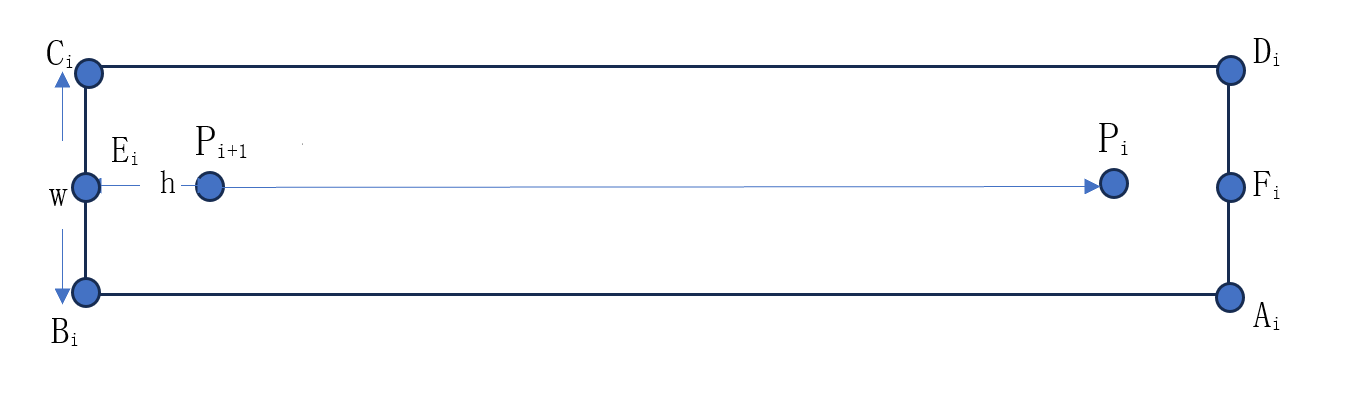
\includegraphics[width=.6\textwidth]{tupian}
    \caption{板凳顶点示意图}
    \label{fig:circuit-diagram}
\end{figure}
\par 设第$i(i=1,2,\cdots,223)$节板凳后把手中心在第$t$秒的直角坐标为$(x_0(t),y_0(t))$,
$(x_i(t),y_i(t))$.设所有板凳的板宽均为$w$,板凳把手中心离最近的板头距离为$h$,则由条件可知$w=0.3m,h=0.275m$.


 \par 记$A_i,B_i,C_i,D_i$在第$t$秒时的位置分别为$A_i(t),B_i(t),C_i(t),D_i(t)$,其直角坐标分别为$(x_{A_i}(t),y_{A_i}(t)),(x_{B_i}(t),y_{B_i}(t)),(x_{C_i}(t),y_{C_i}(t)),(x_{D_i}(t),y_{D_i}(t))$,因此
 \begin{gather}
 \overrightarrow{P_{i+1}\left( t \right) P_i\left( t \right) }=\left( x_i\left( t \right) -x_{i+1}\left( t \right) ,y_i\left( t \right) -y_{i+1}\left( t \right) \right) \label{problem-2.1}
\\
\left| \overrightarrow{A_i\left( t \right) D_i\left( t \right) } \right|=\left| \overrightarrow{B_i\left( t \right) C_i\left( t \right) } \right|=w\label{problem-2.3}
\end{gather}
\par 于是根据向量垂直坐标变换公式可得,对$\forall i\in {0,1,2,\cdots,222}$,都有
\begin{gather}
\overrightarrow{A_i\left( t \right) D_i\left( t \right) }=\overrightarrow{B_i\left( t \right) C_i\left( t \right) }=\left( -\left[ y_i\left( t \right) -y_{i+1}\left( t \right) \right] ,x_i\left( t \right) -x_{i+1}\left( t \right) \right) \label{problem-2.2}
\end{gather}
 \par 对于$B_iC_i$和$A_iD_i$的中点$E_i,F_i$,设它们在第$t$秒时的位置分别为$E_i(t),F_i(t)$,直角坐标分别为
 \begin{align}
    E_i(t)=(x_{E_i}(t),y_{E_i}(t)),\label{1.........20}
    \\
    F_i(t)=(x_{F_i}(t),y_{F_i}(t)).\label{1.........21}
    \end{align}
    从而
    \begin{gather}
    \overrightarrow{P_{i+1}\left( t \right) E_i\left( t \right) }=\left( x_{E_i}\left( t \right) -x_{i+1}\left( t \right) ,y_{E_i}\left( t \right) -x_{i+1}\left( t \right) \right) ,\label{problem-2.4}
    \\
    \overrightarrow{P_i\left( t \right) F_i\left( t \right) }=\left( x_{F_i}\left( t \right) -x_i\left( t \right) ,y_{F_i}\left( t \right) -x_i\left( t \right) \right) ,\label{problem-2.5}
    \\
    \left| \overrightarrow{P_{i+1}\left( t \right) E_i\left( t \right) } \right|=\left| \overrightarrow{P_i\left( t \right) F_i\left( t \right) } \right|=h.\label{problem-2.6}
    \\
    \overrightarrow{E_i\left( t \right) B_i\left( t \right) }=\left( x_{B_i}\left( t \right) -x_{E_i}\left( t \right) ,y_{B_i}\left( t \right) -y_{E_i}\left( t \right) \right) ,\label{problem-2..1}
    \\
    \overrightarrow{E_i\left( t \right) C_i\left( t \right) }=\left( x_{C_i}\left( t \right) -x_{E_i}\left( t \right) ,y_{C_i}\left( t \right) -y_{E_i}\left( t \right) \right) ,\label{problem-2..2}
    \\
    \overrightarrow{F_i\left( t \right) A_i\left( t \right) }=\left( x_{A_i}\left( t \right) -x_{F_i}\left( t \right) ,y_{A_i}\left( t \right) -y_{F_i}\left( t \right) \right) ,\label{problem-2..3}
    \\
    \overrightarrow{F_i\left( t \right) D_i\left( t \right) }=\left( x_{D_i}\left( t \right) -x_{F_i}\left( t \right) ,y_{D_i}\left( t \right) -y_{F_i}\left( t \right) \right) .\label{problem-2..4}
    \end{gather}
    由$E_i,P_i,P_{i+1},F_i$共线可得
    \begin{gather}
    \overrightarrow{P_{i+1}\left( t \right) E_i\left( t \right) }=-\frac{\overrightarrow{P_{i+1}\left( t \right) P_i\left( t \right) }}{\left| \overrightarrow{P_{i+1}\left( t \right) P_i\left( t \right) } \right|}\cdot \left| \overrightarrow{P_{i+1}\left( t \right) E_i\left( t \right) } \right|,\label{problem-2.7}
    \\
    \overrightarrow{P_i\left( t \right) F_i\left( t \right) }=\frac{\overrightarrow{P_{i+1}\left( t \right) P_i\left( t \right) }}{\left| \overrightarrow{P_{i+1}\left( t \right) P_i\left( t \right) } \right|}\cdot \left| \overrightarrow{P_{i+1}\left( t \right) E_i\left( t \right) } \right|.\label{problem-2.8}
    \end{gather}
    联立\eqref{problem-2.1}\eqref{problem-2.4}\eqref{problem-2.5}\eqref{problem-2.6}\eqref{problem-2.7}\eqref{problem-2.8}式可得
    \begin{gather}
    \begin{cases}
    x_{E_i}\left( t \right) =x_{i+1}\left( t \right) -\frac{h}{l_{i+1}}\left( x_i\left( t \right) -x_{i+1}\left( t \right) \right)\\
    y_{E_i}\left( t \right) =y_{i+1}\left( t \right) -\frac{h}{l_{i+1}}\left( y_i\left( t \right) -y_{i+1}\left( t \right) \right)\\
    \end{cases},\label{problem-2.9}
    \\
    \begin{cases}
    x_{F_i}\left( t \right) =x_i\left( t \right) +\frac{h}{l_{i+1}}\left( x_i\left( t \right) -x_{i+1}\left( t \right) \right)\\
    y_{F_i}\left( t \right) =y_i\left( t \right) +\frac{h}{l_{i+1}}\left( y_i\left( t \right) -y_{i+1}\left( t \right) \right)\\
    \end{cases}.\label{problem-2.10}
    \end{gather}
    又由$E_i$是$B_i,C_{i}$的中点和$F_i$是$A_i,D_i$的中点可得
    \begin{gather}
    \overrightarrow{E_i\left( t \right) B_i\left( t \right) }=-\frac{\overrightarrow{B_i\left( t \right) C_i\left( t \right) }}{2},\label{problem-2.11}
    \\
    \overrightarrow{E_i\left( t \right) C_i\left( t \right) }=\frac{\overrightarrow{B_i\left( t \right) C_i\left( t \right) }}{2},\label{problem-2.12}
    \\
    \overrightarrow{F_i\left( t \right) A_i\left( t \right) }=-\frac{\overrightarrow{A_i\left( t \right) D_i\left( t \right) }}{2},\label{problem-2.13}
    \\
    \overrightarrow{F_i\left( t \right) D_i\left( t \right) }=\frac{\overrightarrow{A_i\left( t \right) D_i\left( t \right) }}{2}.   \label{problem-2.14} 
    \end{gather}
    因此联立\eqref{problem-2.2}\eqref{problem-2.3}\eqref{problem-2..1}\eqref{problem-2..2}\eqref{problem-2..3}\eqref{problem-2..4}\eqref{problem-2.9}\eqref{problem-2.10}\eqref{problem-2.11}\eqref{problem-2.12}\eqref{problem-2.13}式,解得板凳的四个顶点坐标。
    \begin{gather}
    \begin{cases}
    x_{A_i}\left( t \right) =x_i\left( t \right) +\frac{h}{l_{i+1}}\left( x_i\left( t \right) -x_{i+1}\left( t \right) \right) +\frac{y_i\left( t \right) -y_{i+1}\left( t \right)}{2}\\ \label{1.........24}
    y_{A_i}\left( t \right) =y_i\left( t \right) +\frac{h}{l_{i+1}}\left( y_i\left( t \right) -y_{i+1}\left( t \right) \right) -\frac{x_i\left( t \right) -x_{i+1}\left( t \right)}{2}\\ 
    \end{cases},
    \\
    \begin{cases}
    x_{B_i}\left( t \right) =x_{i+1}\left( t \right) -\frac{h}{l_{i+1}}\left( x_i\left( t \right) -x_{i+1}\left( t \right) \right) +\frac{y_i\left( t \right) -y_{i+1}\left( t \right)}{2}\\ \label{1.........26}
    y_{B_i}\left( t \right) =y_{i+1}\left( t \right) -\frac{h}{l_{i+1}}\left( y_i\left( t \right) -y_{i+1}\left( t \right) \right) -\frac{x_i\left( t \right) -x_{i+1}\left( t \right)}{2}\\ 
    \end{cases},
    \\
    \begin{cases}
    x_{C_i}\left( t \right) =x_{i+1}\left( t \right) -\frac{h}{l_{i+1}}\left( x_i\left( t \right) -x_{i+1}\left( t \right) \right) -\frac{y_i\left( t \right) -y_{i+1}\left( t \right)}{2}\\ \label{1.........28}
    y_{C_i}\left( t \right) =y_{i+1}\left( t \right) -\frac{h}{l_{i+1}}\left( y_i\left( t \right) -y_{i+1}\left( t \right) \right) +\frac{x_i\left( t \right) -x_{i+1}\left( t \right)}{2}\\ 
    \end{cases},
    \\
    \begin{cases}
    x_{D_i}\left( t \right) =x_i\left( t \right) +\frac{h}{l_{i+1}}\left( x_i\left( t \right) -x_{i+1}\left( t \right) \right) -\frac{y_i\left( t \right) -y_{i+1}\left( t \right)}{2}\\   \label{1.........30}
    y_{D_i}\left( t \right) =y_i\left( t \right) +\frac{h}{l_{i+1}}\left( y_i\left( t \right) -y_{i+1}\left( t \right) \right) +\frac{x_i\left( t \right) -x_{i+1}\left( t \right)}{2}\\   
    \end{cases}.
    \end{gather}
    \noindent\textbf{Step 2 碰撞判断模型}
\par 确定板凳龙盘入发生碰撞前的终止时刻,可以先求解板凳龙何时发生碰撞,并将发生碰撞问题转化为板凳对应的边界有交点的问题。对于任意大于0的时刻 \(t\) ,板凳龙在第 \(t\) 秒发生碰撞的充分必要条件是:存在 \(s\) 和 \(k\) ,且 \(s, k \in \{1, 2, \cdots, 223\}\) ,使得在第 \(t\) 秒时,由 \(A_s(t)\) 、 \(B_s(t)\) 、 \(C_s(t)\) 、 \(D_s(t)\) 所确定的矩形与 \(A_k(t)\) 、 \(B_k(t)\) 、 \(C_k(t)\) 、 \(D_k(t)\) 所确定的矩形存在交点,这意味着对应的两节板凳发生了碰撞。因此,我们的核心任务就转变为在每一秒,对所有可能的 \(i\) 和 \(j\) (\(i, j \in \{1, 2, \cdots, 223\}\) ,$i\ne j$),判断矩形 \(A_i(t)B_i(t)C_i(t)D_i(t)\) 和矩形 \(A_j(t)B_j(t)C_j(t)D_j(t)\) 是否有交点。
\par 为了有效判断两个矩形是否相交,我们借助向量叉乘的性质(详见\href{https://zhuanlan.zhihu.com/p/644689588}{几何算法:判断两条线段是否相交})来设计判定算法。从矩形 \(A_i(t)B_i(t)C_i(t)D_i(t)\) 中任选一条边,记为 \(X_1(t)Y_1(t)\) ,同时从矩形 \(A_j(t)B_j(t)C_j(t)D_j(t)\) 中选取一条边,记为 \(X_2(t)Y_2(t)\) 。
\begin{align}\label{1.........32}
    \begin{cases}
    \text{若}\left( \overrightarrow{X_1\left( t \right) Y_1\left( t \right) }\times \overrightarrow{X_1\left( t \right) X_2\left( t \right) } \right) \cdot \left( \overrightarrow{X_1\left( t \right) Y_1\left( t \right) }\times \overrightarrow{X_1\left( t \right) Y_2\left( t \right) } \right) >0,\text{则判定}\overrightarrow{X_1\left( t \right) Y_1\left( t \right) },
    \\\overrightarrow{X_2\left( t \right) Y_2\left( t \right) }\text{相交}.\\
    \text{若}\left( \overrightarrow{X_1\left( t \right) Y_1\left( t \right) }\times \overrightarrow{X_1\left( t \right) X_2\left( t \right) } \right) \cdot \left( \overrightarrow{X_1\left( t \right) Y_1\left( t \right) }\times \overrightarrow{X_1\left( t \right) Y_2\left( t \right) } \right) \leqslant 0,\text{则判定}\overrightarrow{X_1\left( t \right) Y_1\left( t \right) },
    \\\overrightarrow{X_2\left( t \right) Y_2\left( t \right) }\text{不相交}.\\
    \end{cases}
    \end{align}
    \par 为了准确判断矩形 \(A_i(t)B_i(t)C_i(t)D_i(t)\) 和矩形 \(A_j(t)B_j(t)C_j(t)D_j(t)\) 是否相交,需要将矩形 \(A_i(t)B_i(t)C_i(t)D_i(t)\) 的四条边分别与矩形 \(A_j(t)B_j(t)C_j(t)D_j(t)\) 的四条边按照上述规则进行逐一判断。只有当所有边对判断的结果都显示不相交时,才能确定这两个矩形不存在交点,即两节板凳不发生碰撞;只要存在一组边对判断结果为相交,就可以认定这两个矩形存在交点,即两节板凳发生碰撞。
 \\\noindent\textbf{Step 3 模型求解方法}
\par 首先,我们将初始步长$\varDelta t_0$ 设为 1 秒.然后,从 \(t = 0\) 开始,以步长 $\varDelta t_0$ 进行遍历。在每一个时间点 \(t\) ,对于所有的 \(i \in \{1, 2, \cdots, 223\}\) ,将矩形 \(A_{i}(t)B_{i}(t)C_{i}(t)D_{i}(t)\) 和矩形 \(A_{1}(t)B_{1}(t)C_{1}(t)D_{1}(t)\) 或矩形 \(A_{i}(t)B_{i}(t)C_{i}(t)D_{i}(t)\)分别代入Step 2中的碰撞判断模型判断是否相交。若在当前步长下遍历完所有时间点都未发现碰撞,则对步长进行调整,增加步长时间,然后继续上述步骤。如果在某一时刻 \(t\) ,发现存在相交情况,记录此时的时间 \(t\),确定碰撞时间范围,缩短时间步长为原来的\(\frac{1}{100}\)或\(\frac{1}{10}\) ,在碰撞时间范围内继续进行循环判断。最后,不断调整时间和步长,直到找到舞龙队发生碰撞前的时刻。
 \\\noindent\textbf{Step 4 位置与速度}
\par 将Step 3求得的舞龙队发生碰撞前的时刻代入问题一的模型当中,利用Python求解得到此时板凳龙各把手的位置直角坐标和速度。
\subsubsection{模型计算结果}
\subsection{问题三的模型的建立与求解}
\subsubsection{模型的建立}
\noindent\textbf{Step 1 起始螺距}
\par   记调头空间半径\(R = 4.5m\)。通过问题二,我们已知在螺距为\(55cm\)时,舞龙队盘入的终止时刻(板凳之间不发生碰撞的最晚时刻即$t_1$)龙头前把手的极径$\rho _0(t_1)$,将两者进行对比可知,\(\rho _0(t_1)<R\) ,这表明在该螺距下,舞龙队能够在不发生碰撞的前提下盘入调头空间。
\par 因此,将\(55cm\)作为后续搜寻最小螺距的起始上限值,以此为基础逐步缩小螺距范围。
\\\textbf{Step 2 最小螺距的确定}
\par 为了搜寻到最小螺距,我们进行以下步骤:
\\\noindent\textbf{1.初始螺距和步长的确定}
\par 将\(55cm\)作为初始螺距值,选取\(0.01m\)作为步长开始减小螺距。
\\\noindent\textbf{2.判断是否发生碰撞}
\par 在每一轮计算中,首先确定龙头板凳到达调头空间边界的时间\(t\) 。在时间区间\([0, t]\)内,运用问题二中建立的碰撞判断模型,以此精确判断第$i(i=3,\cdots,223)$节板凳与龙头、第\(2\)块板凳之间是否发生碰撞。
\\\noindent\textbf{3.循环迭代}
\begin{itemize}
\item 若在当前螺距下未检测到碰撞,则确定了螺距的上界,以该螺距为初始值,按照设定步长减小螺距,并再次进行碰撞判断;
\item 若发生碰撞,则确定了螺距的范围,以此螺距为下界,将步长缩小为原来的十分之一(即从\(0.01m\)调整为\(0.001m\) ),在该范围内继续进行碰撞判断.
\end{itemize}
\noindent\textbf{4.终止}
\par 最终,将步长为$10^{-6}$作为循环的终止条件,得到较为精确的满足条件的最小螺距。
\textbf{Step 3 流程图 }

\subsubsection{模型计算结果}
\subsection{问题四的模型的建立与求解}
\subsubsection{模型的建立}
\noindent\textbf{Step 1 分析调头区域}
\par 根据题目要求,舞龙队在调头空间内的运动轨迹大致如下:
\begin{figure}[!h]
    \centering
    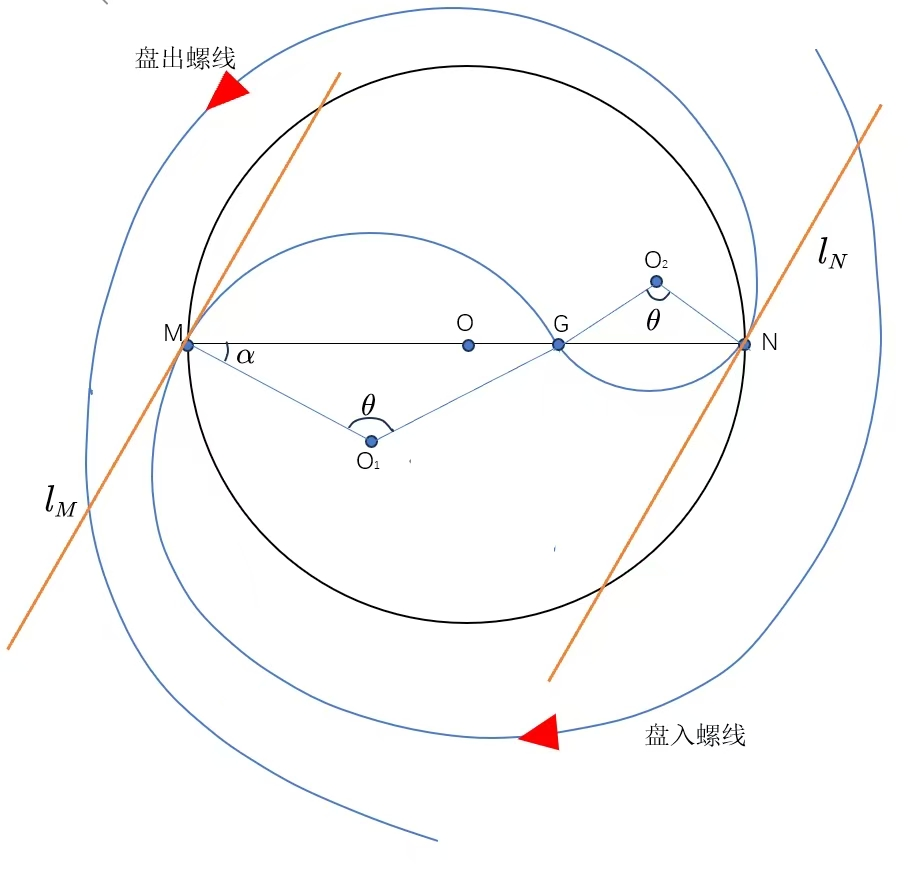
\includegraphics[width=.6\textwidth]{woshiren}
    \caption{调头空间示意图}
  \label{2.2.2.2.2.2} 
\end{figure}
\par 其中,盘入螺线与盘出螺线与调头区域边界交点分别为$M$和$N$。前一段、后一段调头圆弧圆心分别为$O_1$,$O_2$.两段圆弧切点为$G$.过点$M$与盘入螺线相切的直线为$l_M$,过点$N$与盘出螺线相切的直线为$l_N$。记第一段圆弧半径与调头空间直径的夹角为$\alpha $,第一段圆弧对应的夹角为$\theta $。
\\ 根据题目和计算可以得到以下结论:
\begin{itemize}
    \item  由于两段圆弧之间相切,所以$O_1,G,O_2$三点共线。
    \item  经计算可知,$\angle MGO_2+\angle O_2GN=\pi $,基于这个条件,可得M,G,N三点共线。
    \item  因为盘入螺线$\varGamma$与盘出螺线$\varGamma'$中心对称,所以$MN$一定过原点$O$且$l_M$平行于$ l_N$。
    \item  由于两段圆弧均与盘入,盘出螺线相切,因此$O_1M\bot l_M${,}$O_2N\bot l_N$且$O_1M$与$O_2N$的大小比例为2:1。
    \item  由于$O_1M $平行于$ O_2N$,则由几何关系易得
\begin{gather}
\angle MO_1G=\angle NO_2G=\theta,\label{1.........33}
\\
\angle O_1MN=\angle O_1GMN=\angle O_2GN=\angle O_2NG=\alpha .\label{1.........34}
\end{gather}
    \end{itemize} 
    \noindent\textbf{Step 2 证明不可通过改变前后两段调头圆弧半径比例减小调头曲线长度} 
\par 记调头区域半径为$R$,则$\left| \overrightarrow{OM} \right|=\left| \overrightarrow{ON} \right|=R$. 设前后两段调头圆弧半径比例为$a:1$,记后一段调头圆弧的半径为$r$,则前一段调头圆弧的半径为$ar$,其中$a$为任意常数.则
\begin{align}\label{1.........35}
\left| \overrightarrow{O_1M} \right|=\left| \overrightarrow{O_1G} \right|=ar,\left| \overrightarrow{O_2N} \right|=\left| \overrightarrow{O_2G} \right|=r.    
\end{align}
\par 设直线$l_M,$ $l_N,$ $O_1M,$ $MN$的斜率分别为$k_{l_M},$ $k_{l_N},$ $k_{O_1M},$ $k_{MN}$,根据两直线夹角斜率公式可得
\begin{align}\label{1.........36}
\tan \alpha =\tan \angle NMO_1=\frac{k_{MN}-k_{l_M}}{1+k_{MN}k_{l_M}}.
\end{align}
\par 从而
\begin{align}\label{1.........37}
\alpha =\left| \mathrm{arc}\tan \frac{k_{MN}-k_{l_M}}{1+k_{MN}k_{l_M}} \right|.
\end{align}
\par 由\(O_1M\parallel O_2N\),\(\angle MO_1G=\angle NO_2G\) ,\(\angle O_1MG=\angle O_2NG\) ,且\(\vert\overrightarrow{O_1M}\vert = 2\vert\overrightarrow{O_2N}\vert\) ,根据角角边定理可得$\vartriangle MO_1G\cong \vartriangle NO_2G$,由此可得下述线段比例关系
\begin{align}\label{1.........38}
\left| \overrightarrow{NG} \right|=\frac{\left| \overrightarrow{MN} \right|}{1+a}=\frac{2R}{1+a}.
\end{align}
\par 再结合几何关系易得
\begin{align}\label{1.........39}
\theta =\pi -2\alpha ,\quad \cos \alpha =\frac{\frac{1}{2}\left| \overrightarrow{NG} \right|}{\left| \overrightarrow{O_2N} \right|}=\frac{R}{\left( 1+a \right) r}.
\end{align}
\par 因此
\begin{align}\label{1.........40}
r=\frac{R}{\left( 1+a \right) \cos \alpha}.
\end{align}
\par 设$\wideparen{MG}$的长度为$L_1$,$\wideparen{GN}$的长度为$L_2$,记$L=L_1+L_2$.于是根据圆弧长度计算公式可得
\begin{align}\label{equation-1}
L=L_1+L_2=\theta r+\theta ar=\left( 1+a \right) \theta r=\frac{\left( \pi -2\alpha \right) R}{\cos \alpha}=\frac{\left( \pi -2\left| \mathrm{arc}\tan \frac{k_{MN}-k_{l_M}}{1+k_{MN}k_{l_M}} \right| \right) R}{\cos \left| \mathrm{arc}\tan \frac{k_{MN}-k_{l_M}}{1+k_{MN}k_{l_M}} \right|}.
\end{align}
\par 由上式可知$L$与$a$无关,因此不可通过改变前后两段调头圆弧半径比例减小调头曲线长度.

\noindent\textbf{Step 3 调头曲线长度} 
\par 由Step 2可知调头曲线长度与$MN$以及盘入螺线在M处的斜率$l_M$有关,因此我们需要确定$M$,$N$的位置,记它们的极坐标分别为$(\rho_M,\theta_M)$和$(\rho_N,\theta_N)$。由图2可知,$M$与$N$分别为盘入螺线,盘出螺线与调头空间的交点。
\par 其中, 盘入螺线\(\varGamma\)的极坐标方程和直角坐标方程分别为
\begin{gather}
    \varGamma :\rho =\frac{d_0}{2\pi}\theta.\label{7.3.1}
    \\
    \varGamma :\begin{cases}\label{7.4.1}
        x=\frac{d_0}{2\pi}\theta \cos \theta\\
        y=\frac{d_0}{2\pi}\theta \sin \theta\\
        \end{cases}
    \end{gather}
   
    \par 由于盘入螺线与盘出螺线关于螺线中心呈中心对称,因此盘出螺线$\varGamma'$的极坐标方程和直角坐标方程分别为
    \begin{gather}
        \varGamma':\rho =\frac{d_0}{2\pi}\left( \theta +\pi \right) .\label{7.3.2}  \\
        \varGamma':\begin{cases}\label{7.4.2}
            x=\frac{d_0}{2\pi}\left( \theta +\pi \right) \cos \theta\\
            y=\frac{d_0}{2\pi}\left( \theta +\pi \right) \sin \theta\\
            \end{cases}
        \end{gather}
    
    \par 由于调头空间的直径为R,因此其极坐标方程为
    \begin{align}
        S:\rho =R. \label{7.3.3} 
    \end{align}
    \par 因此,将\eqref{7.3.3}式分别与\eqref{7.3.1}式,\eqref{7.3.2}式联立得到$M$,$N$的极坐标
    \begin{gather}\label{1.........40}
        \begin{cases}
        \rho _M=R\\
        \theta _M=\frac{2\pi R}{d_0}\\
        \end{cases}
        \quad,
        \begin{cases}
        \rho _N=R\\
        \theta _N=\frac{2\pi R}{d_0}-\pi \\
        \end{cases}.
        \end{gather}
   \par 通过坐标转化方程,将M,N的极坐标转化为直角坐标
   \begin{gather}\label{1.........42}
    \begin{cases}
        x_M = R\cos\frac{2\pi R}{d_0}\\
        y_M = R\sin\frac{2\pi R}{d_0}\\
    \end{cases}
    \quad,
    \begin{cases}
        x_N = R\cos(\frac{2\pi R}{d_0}-\pi)= - R\cos\frac{2\pi R}{d_0}\\
        y_N = R\sin(\frac{2\pi R}{d_0}-\pi)= - R\sin\frac{2\pi R}{d_0}
         \\
    \end{cases}.
    \end{gather}
    \par 于是得到MN的斜率
    \begin{align}
        k_{MN}=\tan\frac{2\pi R}{d_0}.\label{7.3.4}
        \end{align}
    \par 将\eqref{7.4.1}分别对x和y对于$\theta $求导
    \[
\begin{cases}\label{1.........44}
\frac{dx}{d\theta} = \frac{d_0}{2\pi} (\cos\theta - \theta\sin\theta) \\
\frac{dy}{d\theta} = \frac{d_0}{2\pi} (\sin\theta + \theta\cos\theta)
\end{cases}
\]
\par 于是就有
\begin{align}\label{1.........45}
    \k_{l_M}=\frac{\mathrm{d}y}{dx}\mid_{M}^{}=\frac{\mathrm{d}y/\mathrm{d}\theta}{dx/\mathrm{d}\theta}\mid_{M}^{}=\frac{\sin \theta +\theta \cos \theta}{\cos \theta -\theta \sin \theta}\mid_{\theta =\theta _M}^{}=\frac{\sin\frac{2\pi R}{d_0}+\frac{2\pi R}{d_0}\cos\frac{2\pi R}{d_0}}{\cos\frac{2\pi R}{d_0}-\frac{2\pi R}{d_0}\sin\frac{2\pi R}{d_0}}
\end{align}
\par 所以将\eqref{7.3.4}\eqref{7.4.3}代入可得
\begin{align}\label{1.........46}
 L=.
    \end{align}
\noindent\textbf{Step 4 计算圆心和切点的坐标}     
\begin{enumerate}
\item \textbf{切点坐标}
\end{enumerate} 
\par 通过题目给定条件,我们可以知道,前一段圆弧的半径是后一段的2倍,又由于$\vartriangle MO_1G\cong \vartriangle NO_2G$,所以$\vec{MG}=2\vec{GN}$,记G的直角坐标为$(x_{G},y_{G})$
\begin{gather}\label{1.........47}
\overrightarrow{MG}=\left( x_G-x_M,y_G-y_M \right) ,
\\
\overrightarrow{GN}=\left( x_N-x_G,y_N-y_G \right) .
\end{gather}
\par 在Step 3中我们已经求出M,N的直角坐标,因此
\begin{align}\label{1.........48}
    \begin{cases}
    x_G= -\frac{1}{3}R\cos\frac{2\pi R}{d_0}\\
    y_G=-\frac{1}{3}R\sin\frac{2\pi R}{d_0}\\
    \end{cases}.
    \end{align}
    \begin{enumerate}[start=2]
        \item \textbf{圆心坐标}
        \end{enumerate}   
    \par 设前一段调头圆弧圆心$O_1$的直角坐标与极坐标分别为$(x_{O_1},y_{O_1})$和$(\rho_{O_1},\theta_{O_1})$,后一段调头圆弧圆心$O_2$的直角坐标为$(x_{O_2},y_{O_2})$和$(\rho_{O_2},\theta_{O_2})$.前一段圆弧的半径为$2r$,后一段圆弧的半径为r,因为圆心到圆上任意一点的距离相同,因此
    \begin{gather}\label{1.........49}
        |\overrightarrow{O_1O_2}|= |\overrightarrow{O_1G}| + |\overrightarrow{O_2G}| = 3r\\
	|\overrightarrow{O_1M}|=2r   \\
	|\overrightarrow{O_2M}|=r
 \end{gather}
\par 即
\begin{gather}
    2R=\left| \overrightarrow{MN} \right|=\left| \overrightarrow{MG} \right|+\left| \overrightarrow{GN} \right|= 2r\cos\alpha\times2 + r\cos\alpha\times2 = 6r\cos\alpha,
    \\
    \begin{cases}\label{1.........50}
    \left( x_M-x_{O_1} \right) ^2+\left( y_M-y_{O_1} \right) ^2=4r^2\\
    \left( x_G-x_{O_1} \right) ^2+\left( y_G-y_{O_1} \right) ^2=4r^2\\
    \end{cases},
    \\
    \begin{cases}\label{1.........51}
    \left( x_N-x_{O_2} \right) ^2+\left( y_N-y_{O_2} \right) ^2=r^2\\
    \left( x_G-x_{O_2} \right) ^2+\left( y_G-y_{O_2} \right) ^2=r^2\\
    \end{cases}.
    \end{gather}
        \par 由上式解得
        \begin{gather}\label{1.........52}
        \begin{cases}
        x_{O_1}=\\
        y_{O_1}=\\
        \end{cases},\quad \begin{cases}
        x_{O_2}=\\
        y_{O_2}=\\
        \end{cases}.
    \end{gather}
   \par  进而得到
    \begin{gather}\label{1.........53}
    \begin{cases}
    \rho _{O_1}=\sqrt{x_{O_1}^{2}+y_{O_1}^{2}}=\\
    \theta _{O_1}=\mathrm{arc}\tan \frac{y_{O_1}}{x_{O_1}}=\\
    \end{cases},\quad \begin{cases}
    \rho _{O_2}=\sqrt{x_{O_2}^{2}+y_{O_2}^{2}}=\\
    \theta _{O_2}=\mathrm{arc}\tan \frac{y_{O_2}}{x_{O_2}}=\\
    \end{cases}.
    \end{gather}
    \noindent\textbf{Step 5 计算龙头前把手在各时刻的位置} 
    
\textbf{
    \begin{enumerate}
        \item \textbf{$P_0$位于盘入螺线$\varGamma$上}
        \end{enumerate}  
        }
        \par 当$t\in[-100,0]$时,$P_0$位于盘入螺线$\varGamma$上.从ts至0s,龙头前把手运动的路径长度为$\left( -t \right) v_0$,极角从$\theta _{P_0\left( t \right)} $变为$\theta _M$ ,由第一型曲线积分计算公式可得,曲线$\wideparen{P_0M}$长度
        \begin{align}\label{1.........54}
            S=\left( -t \right) v_0=\int_{\wideparen{P_0M}}{\mathrm{d}s}=\int_{\theta _M}^{\theta _{P_0\left( t \right)}}{\sqrt{\left[ \rho _{\varGamma}\left( \theta \right) \right] ^2+\left[ \rho _{\varGamma}^{\prime}\left( \theta \right) \right] ^2}\mathrm{d}\theta}=\frac{d_0}{2\pi}\int_{\theta _M}^{\theta _{P_0\left( t \right)}}{\sqrt{{\theta}^2+1}\mathrm{d}\theta}.
        \end{align}
       
        
        \par 通过求解,可以得到龙头前把手某一时间点与其极角之间的关系
        \begin{align}\label{1.........55}
            (-t)v_0=\frac{d_0}{4\pi}\left[\theta_{P_0(t)}\sqrt{\theta_{P_0(t)}^2 + 1}+\ln(\theta_{P_0(t)}+\sqrt{\theta_{P_0(t)}^2 + 1})-\theta_M\sqrt{\theta_M^2 + 1}-\ln(\theta_M+\sqrt{\theta_M^2 + 1})\right]
        \end{align}
        
        由上式解得$P_0$的极角,再通过\eqref{0.1}可以求得$P_0$的极坐标,通过坐标转化方程\eqref{0.0}求得$P_0$在直角坐标系下的坐标.

        \textbf{
       \begin{enumerate}[start=2]
        \item \textbf {$P_0$位于调头曲线$\wideparen{MG}$上}
        \end{enumerate}    
            }
      \par   当$t\in[0,\frac{L_1}{v_0}]$时,\(P_{0}\)在以\(O_{1}\)为圆心,半径为\(2r\)的圆弧\(\wideparen{MG}\)上运动,且运动速度为\(v_{0}\),在时间\(t\)内,\(P_{0}\)所经过的弧长对应的圆心角为\(\angle P_{0}(t)O_{1}M\)。根据弧长公式\(l = \alpha r\),可得
\begin{align}
        v_{0}t = \angle P_{0}(t)O_{1}M \cdot 2r \label{7.5.1}
\end{align} 
\par 根据直线斜率的定义,直线\(O_{1}M\)的斜率\(k_{O_{1}M}\),\(O_{1}P_{0}(t)\)的斜率\(k_{O_{1}P_{0}(t)}\)为

        \begin{align}\label{1.........57}
        k_{O_1M}=\frac{y_{O_1}-y_M}{x_{O_1}-x_M},k_{O_1P_0\left( t \right)}=\frac{y_{O_1}-y_{P_0\left( t \right)}}{x_{O_1}-x_{P_0\left( t \right)}},
        \end{align}
        \par 依据两直线夹角的正切公式,\(\angle P_{0}(t)O_{1}M\)的正切值为
\begin{align}
        \tan\angle P_{0}(t)O_{1}M = \frac{k_{O_{1}M} - k_{O_{1}P_{0}(t)}}{1 + k_{O_{1}M}k_{O_{1}P_{0}(t)}} \in [0, \pi] \label{7.5.2}
\end{align}
\par 联立\eqref{7.5.1}\eqref{7.5.2},得到
        \begin{align}
      \tan \frac{v_0t}{2r}=\tan \angle P_0\left( t \right) O_1M=\frac{k_{O_1M}-k_{O_1P_0\left( t \right)}}{1+k_{O_1M}k_{O_1P_0\left( t \right)}}=\frac{\frac{y_{O_1}-y_M}{x_{O_1}-x_M}-\frac{y_{O_1}-y_{P_0\left( t \right)}}{x_{O_1}-x_{P_0\left( t \right)}}}{1+\frac{y_{O_1}-y_M}{x_{O_1}-x_M}\frac{y_{O_1}-y_{P_0\left( t \right)}}{x_{O_1}-x_{P_0\left( t \right)}}},\label{7.5.3}
         \end{align}
\par 由于$P_{0}(t)$到圆心$O_{1}$的距离始终等于圆弧半径\(2r\),根据两点间距离公式,可得
\begin{align}
(x_{O_{1}} - x_{P_{0}(t)})^{2} + (y_{O_{1}} - y_{P_{0}(t)})^{2} = 4r^{2} \label{7.5.4}
\end{align} 

\par 因此,通过\eqref{7.5.3}\eqref{7.5.4}解得$P_0$的位置坐标.

\textbf{
\begin{enumerate}[start=3]
    \item \textbf {$P_0$位于调头曲线$\wideparen{GN}$上}
    \end{enumerate}    
 }       
        当$t\in[\frac{L_1}{v_0},\frac{L}{v_0}]$时,\(P_{0}\)在以\(O_{2}\)为圆心,半径为\(r\)的圆弧\(\wideparen{GN}\)上运动,且运动速度为\(v_{0}\),在时间$t-\frac{L_1}{v_0}$内,\(P_{0}\)所经过的弧长对应的圆心角为\(\angle P_{0}(t)O_{2}G\)。根据弧长公式\(l = \alpha r\),可得
\begin{align}
    v_0\left( t-\frac{L_1}{v_0} \right) =\angle P_0\left( t \right) O_2G\cdot r,\label{7.5.5}
\end{align} 
\par 根据直线斜率的定义,直线\(O_{2}G\)的斜率\(k_{O_{2}G}\),\(O_{2}P_{0}(t)\)的斜率\(k_{O_{2}P_{0}(t)}\)为

        \begin{align}
            k_{O_2G}=\frac{y_{O_2}-y_G}{x_{O_2}-x_G},k_{O_2P_0\left( t \right)}=\frac{y_{O_2}-y_{P_0\left( t \right)}}{x_{O_2}-x_{P_0\left( t \right)}},\label{7.5.6}
        \end{align}
        \par 依据两直线夹角的正切公式,\(\angle P_{0}(t)O_{2}G\)的正切值为
\begin{align}
    \tan \angle P_0\left( t \right) O_2G=\frac{k_{O_2G}-k_{O_2P_0\left( t \right)}}{1+k_{O_2G}k_{O_2P_0\left( t \right)}}\in \left[ 0,\pi \right] ,\label{7.5.6}
\end{align}
\par 联立\eqref{7.5.5}\eqref{7.5.6},得到
        \begin{align}
            \tan \frac{v_0\left( t-\frac{L_1}{v_0} \right)}{r}=\tan \angle P_0\left( t \right) O_2G=\frac{k_{O_2G}-k_{O_2P_0\left( t \right)}}{1+k_{O_2G}k_{O_2P_0\left( t \right)}}=\frac{\frac{y_{O_2}-y_G}{x_{O_2}-x_G}-\frac{y_{O_2}-y_{P_0\left( t \right)}}{x_{O_2}-x_{P_0\left( t \right)}}}{1+\frac{y_{O_2}-y_G}{x_{O_2}-x_G}\frac{y_{O_2}-y_{P_0\left( t \right)}}{x_{O_2}-x_{P_0\left( t \right)}}},\label{7.5.7}
        \end{align}
\par 由于$P_{0}(t)$到圆心$O_{2}$的距离始终等于圆弧半径\(r\),根据两点间距离公式,可得
\begin{align}
    \left( x_{O_2}-x_{P_0\left( t \right)} \right) ^2+\left( y_{O_2}-y_{P_0\left( t \right)} \right) ^2=r^2.\label{7.5.8}
\end{align} 

\par 因此,通过\eqref{7.5.7}\eqref{7.5.8}解得$P_0$的位置坐标.  

\begin{enumerate}[start=4]
    \item \textbf{$P_0$位于盘出螺线$\varGamma'$上}
    \end{enumerate}  
    \par 当$t\in[\frac{L}{v_0},100]$时,$P_0$位于盘入螺线$\varGamma'$上.从$\frac{L}{v_0}$至ts,龙头前把手运动的路径长度为$v_0\left( t-\frac{L}{v_0} \right)$,极角从$\theta _N$变为$\theta _{P_0\left( t \right)} $ ,由第一型曲线积分计算公式可得,曲线$\wideparen{P_0M}$长度
    \begin{small}
    \begin{align}\label{1.........441}
        S=v_0\left( t-\frac{L}{v_0} \right) =\int_{P_0\left( t \right) N}{\mathrm{d}s}=\int_{\theta _N}^{\theta _{P_0\left( t \right)}}{\sqrt{\left[ \rho _{\varGamma \prime}\left( \theta \right) \right] ^2+\left[ \rho _{\varGamma \prime}^{\prime}\left( \theta \right) \right] ^2}\mathrm{d}\theta}=\frac{d_0}{2\pi}\int_{\theta _N}^{\theta _{P_0\left( t \right)}}{\sqrt{\left( \theta +\pi \right) ^2+1}\mathrm{d}\theta }.
    \end{align}
\end{small}
    \par 通过求解,可以得到龙头前把手某一时间点与其极角之间的关系
   \begin{small}
        \begin{align*}\label{1.........442}
        &\frac{d_0}{4\pi}\left[( \theta_{P_0}(t)+\pi)\sqrt{(\theta_{P_0}(t)+\pi)^{2}+1}-(\theta_N+\pi)\sqrt{(\theta_N+\pi)^{2}+1}+\ln\frac{\theta_{P_0}(t)+\pi+\sqrt{(\theta_{P_0}(t)+\pi)^{2}+1}}{\theta_N+\pi+\sqrt{(\theta_N+\pi)^{2}+1}}\right]
        \end{align*}
    \end{small}
    
    \par 由上式解得$P_0$的极角,再通过\eqref{0.1}可以求得$P_0$的极坐标,通过坐标转化方程\eqref{0.0}求得$P_0$在直角坐标系下的坐标.
\\\noindent\textbf{Step 6 计算板凳龙从-100s到100s其余各把手的位置} 


\par 当$t\in[-100,100]$时,板凳龙部分把手位于调头曲线上,此时需要对板凳龙的运动轨迹分段处理,我们将板凳龙的运动轨迹分为盘入螺线$\varGamma$、前一段调头曲线$\wideparen{MG}$、后一段调头曲线$\wideparen{GN}$、盘出螺线$\varGamma'$四段.
然后我们需要根据前一个把手的位置判断与其相邻的后一个把手所在的轨迹曲线,进而递推解出后一个把手的位置.
\textbf{
\begin{enumerate}
   \item  情形1:板凳龙在盘入螺线$\varGamma$上
\end{enumerate}
}
\par 当第$t$秒,$P_i(0\leq i\leq 222)$在盘入螺线$\varGamma$上时,利用问题1的模型求解$P_{i+1}$的直角坐标即可.
\textbf{
\begin{enumerate}[start=2]
    \item  情形2:板凳龙在调头曲线$\wideparen{MG}$上 \label{7.6.1}
 \end{enumerate}
}
\begin{itemize}
\item \textbf{引入判断角$\beta_1$}
\end{itemize}






\par 当第$t$秒$P_i(0\leq i\leq 222)$在$\wideparen{MG}$上时,引入判断角.若$P_{i+1}$与$M$点重合,则定义此时$\angle P_iO_1P_{i+1}=\beta_1$,称$\beta_1$为$\wideparen{MG}$判断角. 几何示意图如下:
\begin{figure}[!h]
    \centering
    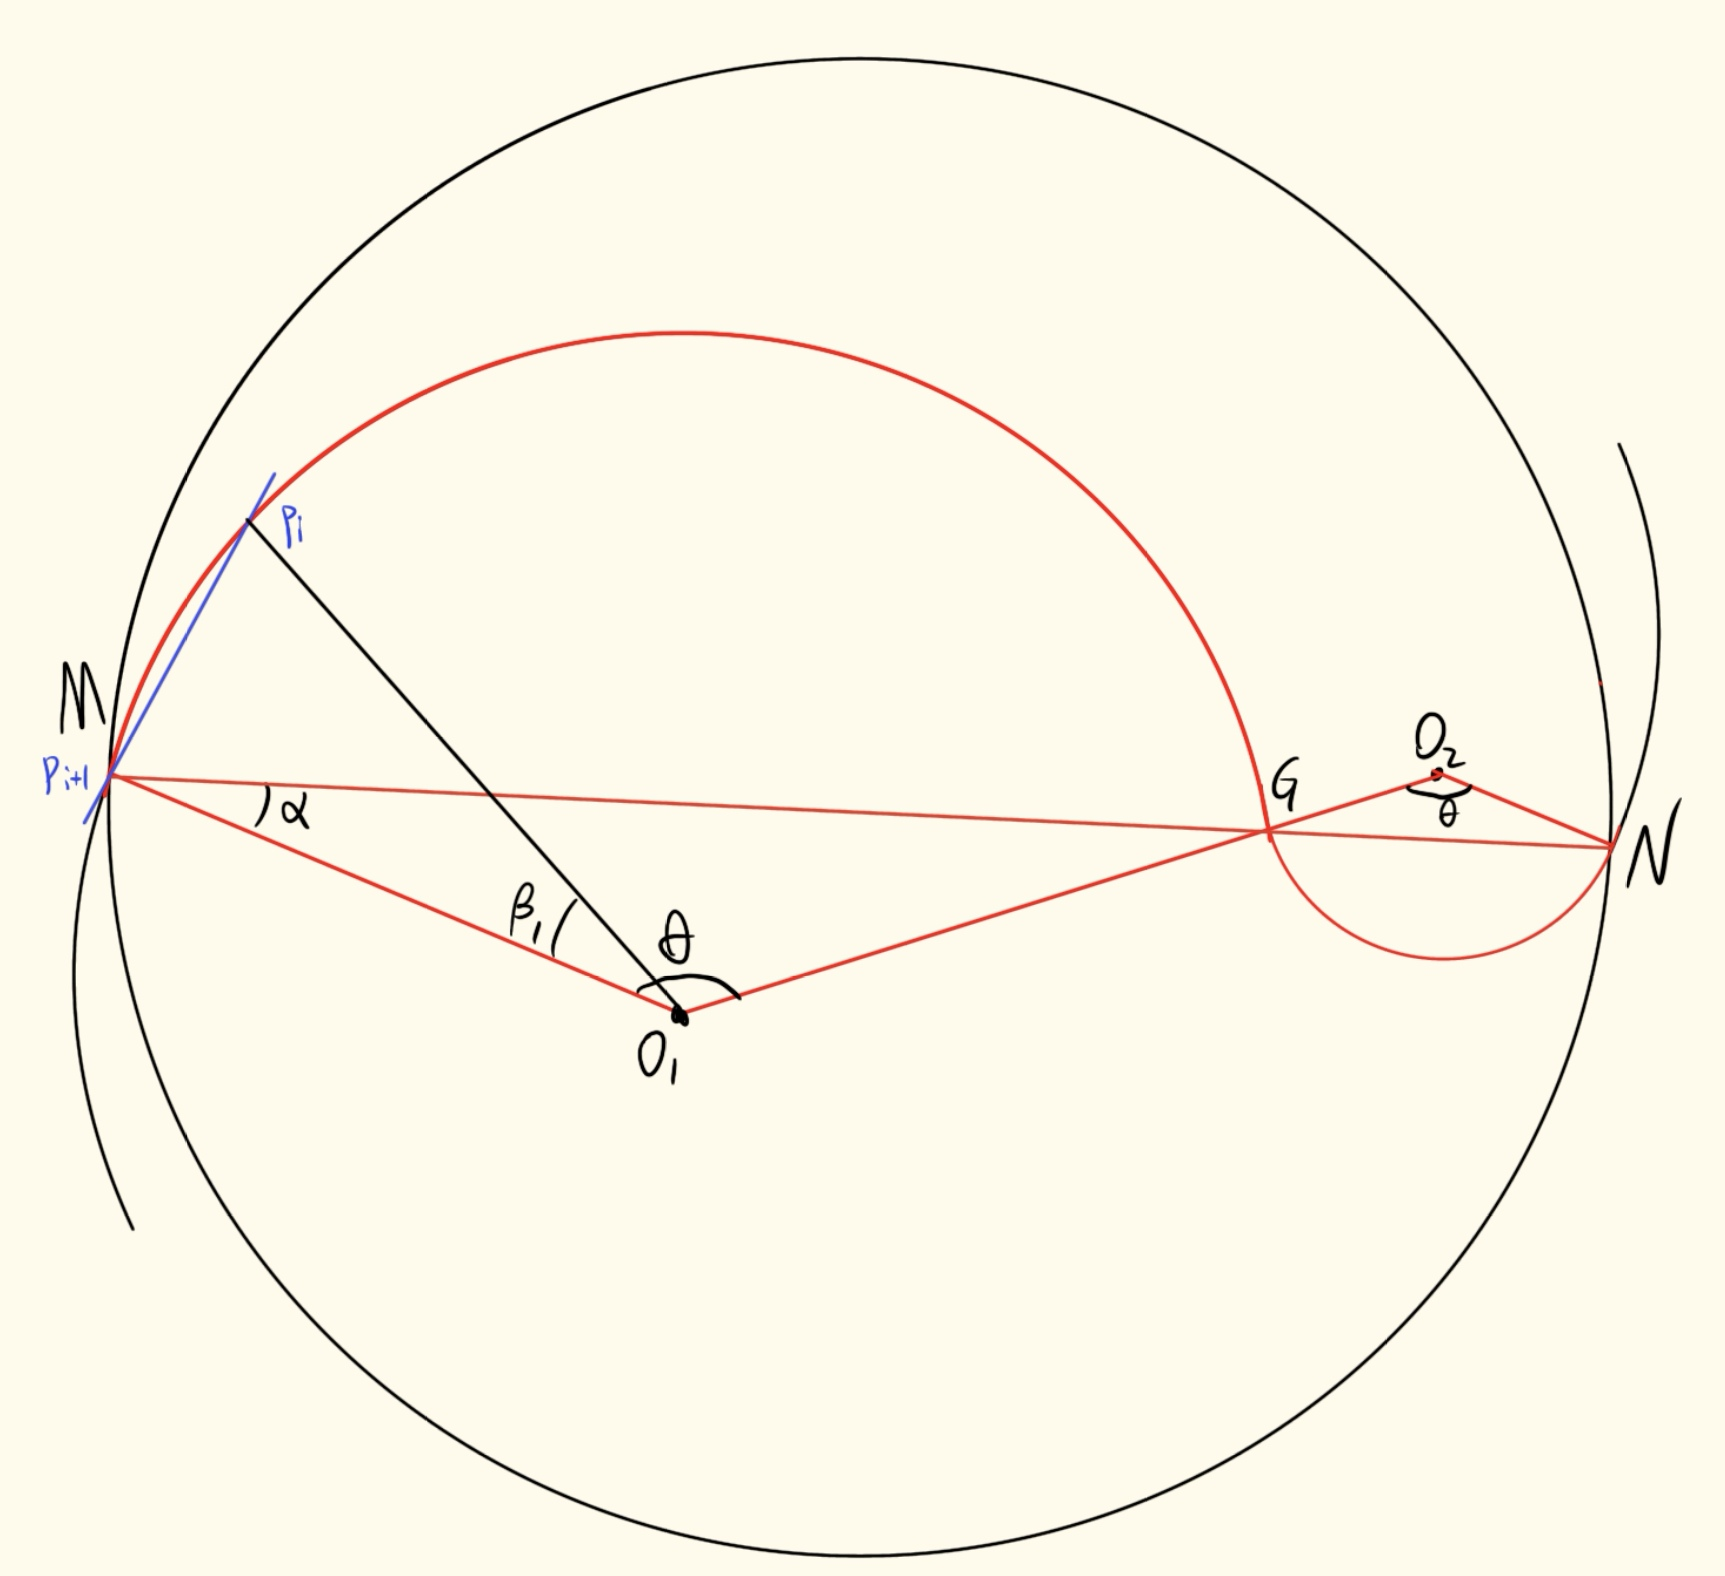
\includegraphics[width=.6\textwidth]{几何示意图1}
    \caption{几何示意图1}
\end{figure}
\par 在由点 \(P_{i}\)、\(O_{1}\) 和 \(P_{i + 1}\) 构成的三角形中,根据余弦定理有
\begin{align}
l_{i+1}^{2}=\left| \overrightarrow{P_iP_{i+1}} \right|^2=4r^2-4r^2\cos \beta _1.
\end{align}
由上式解得
\begin{align}\label{1.........443}
\beta _1=\left| \mathrm{arc}\cos \left( 1-\frac{l_{i+1}^{2}}{4r^2} \right) \right|=.
\end{align}
\begin{itemize}
    \item \textbf{计算$\angle P_{i}(t)O_1M$}
    \end{itemize}
    

根据几何关系及两直线夹角斜率公式可得
\begin{gather}\label{1.........444}
k_{O_1M}=\frac{y_M-y_{O_1}}{x_M-x_{O_1}},k_{O_1P_i\left( t \right)}=\frac{y_{P_i\left( t \right)}-y_{O_1}}{x_{P_i\left( t \right)}-x_{O_1}},
\\
\tan \angle P_i(t)O_1M=\frac{k_{O_1M}-k_{O_1P_i\left( t \right)}}{1+k_{O_1M}k_{O_1P_i\left( t \right)}}.
\end{gather}
\par 从而
\begin{align}\label{1.........445}
\angle P_i(t)O_1M= \mathrm{arc}\tan \frac{\frac{y_M-y_{O_1}}{x_M-x_{O_1}}-\frac{y_{P_i\left( t \right)}-y_{O_1}}{x_{P_i\left( t \right)}-x_{O_1}}}{1+\frac{y_M-y_{O_1}}{x_M-x_{O_1}}\cdot \frac{y_{P_i\left( t \right)}-y_{O_1}}{x_{P_i\left( t \right)}-x_{O_1}}}\in[0,\pi].
\end{align}
\begin{itemize}
    \item \textbf{判断并计算$P_{i+1}$的位置}\label{subsubsection4.4.1.2}
\end{itemize}
    \par 在得到\(\angle P_{i}(t)O_{1}M\) 和\(\beta_{1}\) 后,我们通过比较它们的大小来判断 \(P_{i + 1}\) 的位置.
    \par 若\(\angle P_{i}(t)O_{1}M \geq \beta_{1}\) ,根据几何关系可知,\(P_{i + 1}\) 一定位于圆弧\(\wideparen{MG}\) 上。此时,我们可以根据以下两个方程来确定 \(P_{i + 1}\) 的坐标:
    \begin{align}\label{1.........446}
        \left\{ \begin{array}{c}
        \left( x_{i+1}-x_i \right) ^2+\left( y_{i+1}-y_i \right) ^2=l_{i+1}^{2}\\
        \left( x_{i+1}-x_{O_1} \right) ^2+\left( y_{i+1}-y_{O_1} \right) ^2=4r^2\\
        \end{array} \right. .
        \end{align}
\par 联立这两个方程求解,会得到\((x_{i + 1}, y_{i + 1})\) 的多个可能解。但结合题意可知,在这些解中,\(x_{i + 1}\) 的真实解是其中最小的一个,由此我们就能确定 \(P_{i + 1}\) 的直角坐标\((x_{i + 1}, y_{i + 1})\) .
\par 若$\angle P_i(t)O_1M< \beta_1$,则$P_{i+1}$一定位于盘入螺线$\varGamma$上.此时,我们利用问题1中建立的模型,按照相应的计算方法解出\((x_{i + 1}, y_{i + 1})\) 即可.


\textbf{
\begin{enumerate}[start=2]
    \item  情形3:板凳龙在调头曲线$\wideparen{GN}$上
 \end{enumerate}
}
\begin{itemize}
\item \textbf{引入判断角$\beta_2$}
\end{itemize}

\par 当第$t$秒$P_i(0\leq i\leq 222)$在$\wideparen{GN}$上时,引入判断角.若$P_{i+1}$与$G$点重合,则定义此时$\angle P_iO_1P_{i+1}=\beta_2$,称$\beta_2$为$\wideparen{GN}$判断角. 几何示意图如下:
\begin{figure}[!h]
    \centering
    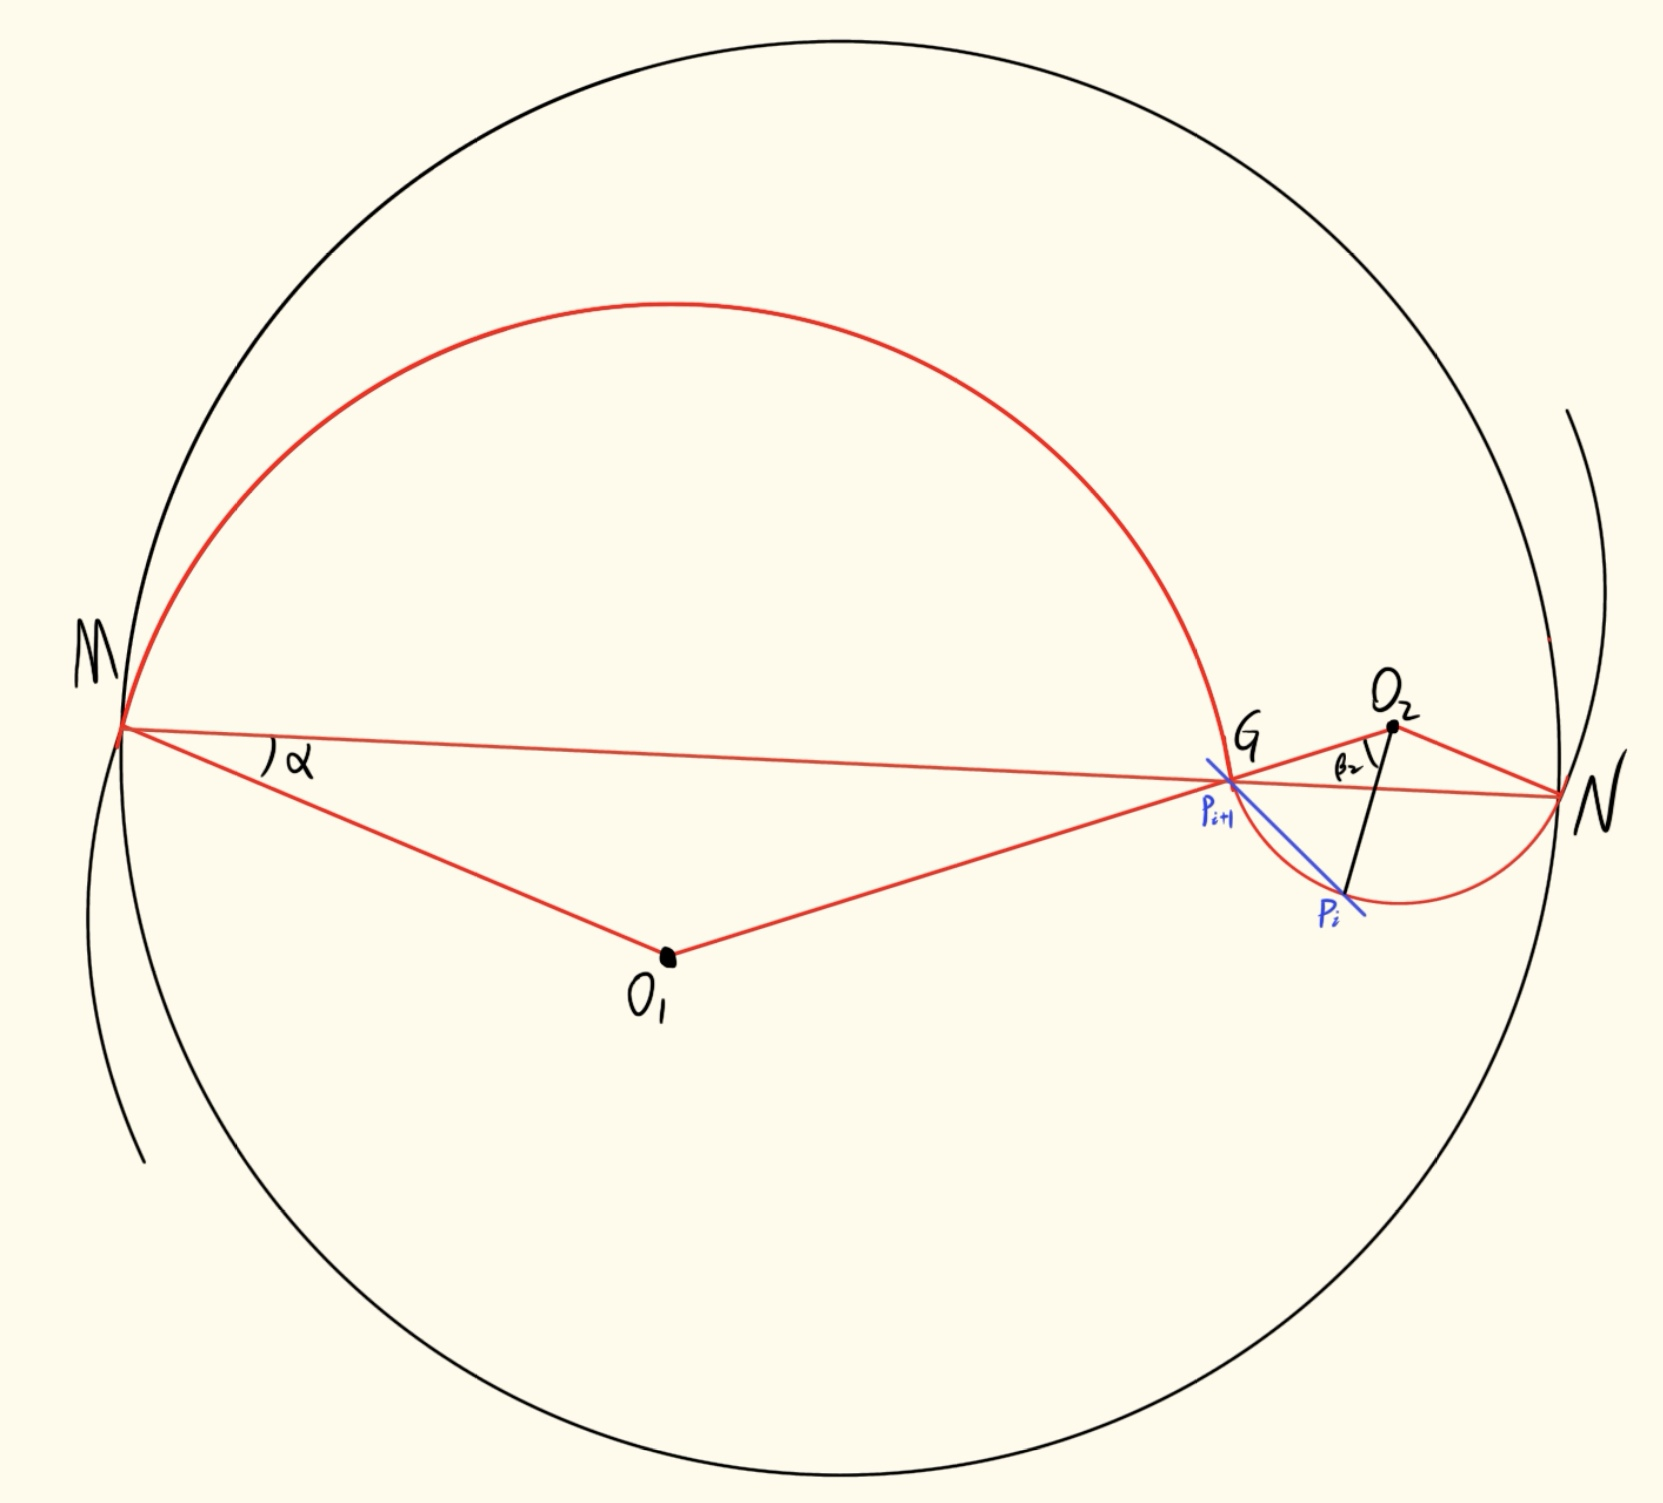
\includegraphics[width=.6\textwidth]{几何示意图2}
    \caption{几何示意图2}
\end{figure}
\par 在由点$ P_{i}、O_{1} $和 $P_{i + 1} $构成的三角形中,根据余弦定理有
\begin{align}\label{1.........448}
l_{i+1}^{2}=\left| \overrightarrow{P_iP_{i+1}} \right|^2=2r^2-2r^2\cos \beta _2.
\end{align}
由上式解得
\begin{align}\label{1.........449}
\beta _2=\left| \mathrm{arc}\cos \left( 1-\frac{l_{i+1}^{2}}{2R^2} \right) \right|=.
\end{align}

\begin{itemize}
    \item \textbf{计算$\angle P_{i}(t)O_2G$}
    \end{itemize}

\par 根据几何关系及两直线夹角斜率公式可得
\begin{gather}\label{1.........450}
k_{O_1O_2}=\frac{y_{O_2}-y_{O_1}}{x_{O_2}-x_{O_1}},k_{O_2P_i\left( t \right)}=\frac{y_{P_i\left( t \right)}-y_{O_2}}{x_{P_i\left( t \right)}-x_{O_2}},
\\
\tan \angle P_i(t)O_2G=\frac{k_{O_1O_2}-k_{O_2P_i\left( t \right)}}{1+k_{O_1O_2}k_{O_2P_i\left( t \right)}}.
\end{gather}
\par 从而
\begin{align}\label{1.........451}
\angle P_i(t)O_2G=\mathrm{arc}\tan \frac{\frac{y_{O_2}-y_{O_1}}{x_{O_2}-x_{O_1}}-\frac{y_{P_i\left( t \right)}-y_{O_2}}{x_{P_i\left( t \right)}-x_{O_2}}}{1+\frac{y_{O_2}-y_{O_1}}{x_{O_2}-x_{O_1}}\frac{y_{P_i\left( t \right)}-y_{O_2}}{x_{P_i\left( t \right)}-x_{O_2}}}\in[0,\pi].
\end{align}
\begin{itemize}
    \item \textbf{判断并计算$P_{i+1}$的位置}
\end{itemize}
\par 在得到$\angle P_{i}(t)O_{2}G $和$\beta_{2} $后,通过比较它们的大小来判断 $P_{i + 1} $的位置。
 
\par 若$\angle P_{i}(t)O_{2}G \geq \beta_{2}$ ,根据几何关系可知,$P_{i + 1}$ 一定位于圆弧$\wideparen{GN} $上。此时,我们可以根据以下两个方程来确定 $P_{i + 1} $的坐标
\begin{align}\label{1.........452}
\left\{ \begin{array}{c}
\left( x_{i+1}-x_i \right) ^2+\left( y_{i+1}-y_i \right) ^2=l_{i+1}^{2}\\
\left( x_{i+1}-x_{O_2} \right) ^2+\left( y_{i+1}-y_{O_2} \right) ^2=r^2\\
\end{array} \right. .
\end{align}
 
\par 联立这两个方程求解,会得到$(x_{i + 1}, y_{i + 1}) $的多个可能解。由题意可知,$x_{i + 1} $的真实解是其中最小的一个。通过这种方式,我们确定了$P_{i + 1} $的直角坐标$(x_{i + 1}, y_{i + 1})$ 。
\par 若$\angle P_i(t)O_2G< \beta_2$,则$P_{i+1}$一定位于圆弧$\wideparen{MG}$上.从而利用情形二解出$(x_{i+1},y_{i+1})$即可.

\textbf{
\begin{enumerate}[start=2]
    \item  情形3:板凳龙在盘出螺线$\varGamma'$上
 \end{enumerate}
}
\begin{itemize}
    \item \textbf{引入判断角$\beta_3$}
    \end{itemize}

\par 当第$t$秒$P_i(0\leq i\leq 222)$在$、\varGamma'$上时,引入判断角.若$P_{i+1}$与$N$点重合,则定义此时$\angle P_iO_2N=\beta_3$,称$\beta_3$为$\varGamma'$判断角. 几何示意图如下:
\begin{figure}[!h]
    \centering
    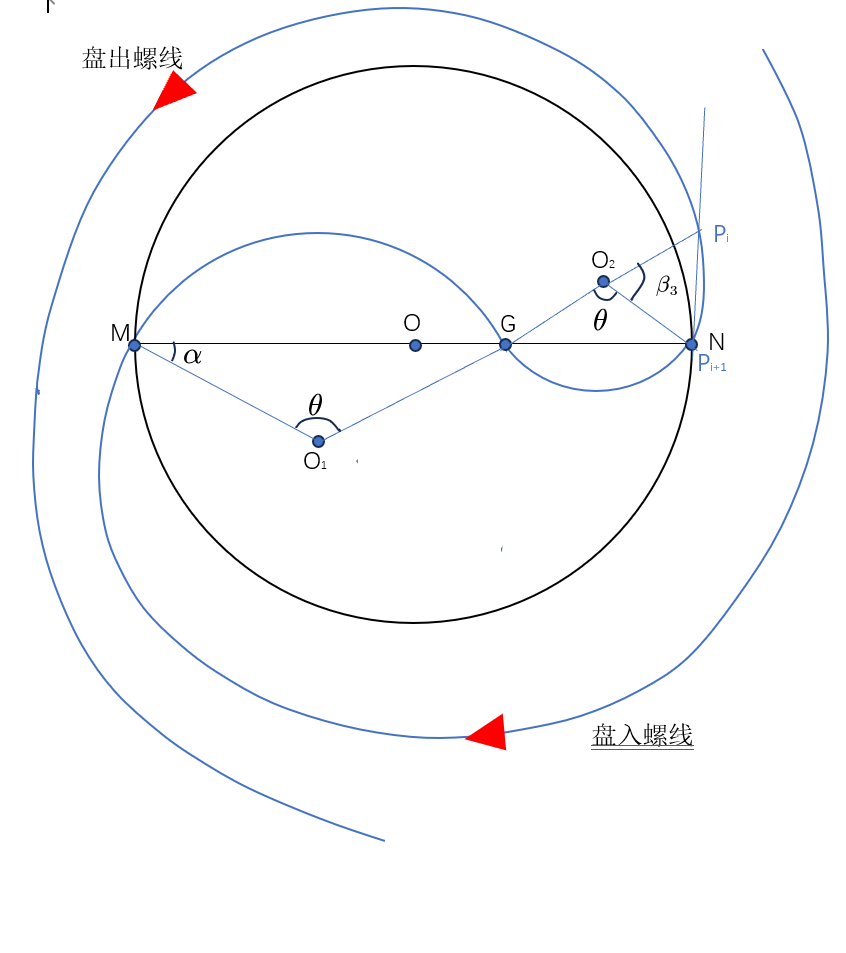
\includegraphics[width=.6\textwidth]{几何示意图3}
    \caption{几何示意图3}
\end{figure}
\par 在由点 \(P_{i}\)、\(O_{2}\) 和 \(P_{i + 1}\) 构成的三角形中,根据余弦定理有

\begin{gather}\label{1.........454}
\left| \overrightarrow{O_2P_i} \right|=\sqrt{\left( x_{P_i}-x_{O_2} \right) ^2+\left( y_{P_i}-y_{O_2} \right) ^2},
\\
l_{i+1}^{2}=\left| \overrightarrow{P_iP_{i+1}} \right|^2=\left| \overrightarrow{O_2P_i} \right|^2+r^2-2r\left| \overrightarrow{O_2P_i} \right|\cos \beta _3.
\end{gather}
由上式解得
\begin{align}\label{1.........455}
\beta _3=\left| \mathrm{arc}\cos \frac{r^2+\left( x_{P_i}-x_{O_2} \right) ^2+\left( y_{P_i}-y_{O_2} \right) ^2-l_{i+1}^{2}}{2r\sqrt{\left( x_{P_i}-x_{O_2} \right) ^2+\left( y_{P_i}-y_{O_2} \right) ^2}} \right|=.
\end{align}

\begin{itemize}
    \item \textbf{计算$\angle P_{i}(t)O_2N$}
    \end{itemize}

\par 根据几何关系及两直线夹角斜率公式可得
\begin{gather}\label{1.........456}
k_{O_2N}=\frac{y_{O_2}-y_N}{x_{O_2}-x_N},k_{O_2P_i\left( t \right)}=\frac{y_{P_i\left( t \right)}-y_{O_2}}{x_{P_i\left( t \right)}-x_{O_2}},
\\
\tan \angle P_i(t)O_2N=\frac{k_{O_2N}-k_{O_2P_i\left( t \right)}}{1+k_{O_2N}k_{O_2P_i\left( t \right)}}.
\end{gather}
从而
\begin{align}\label{1.........457}
\angle P_i(t)O_2N=\mathrm{arc}\tan \frac{\frac{y_{O_2}-y_N}{x_{O_2}-x_N}-\frac{y_{P_i\left( t \right)}-y_{O_2}}{x_{P_i\left( t \right)}-x_{O_2}}}{1+\frac{y_{O_2}-y_N}{x_{O_2}-x_N}\frac{y_{P_i\left( t \right)}-y_{O_2}}{x_{P_i\left( t \right)}-x_{O_2}}}\in \left[ 0,\pi \right] .
\end{align}
\begin{itemize}
    \item \textbf{判断并计算$P_{i+1}$的位置}
    \end{itemize}
    \par 在得到$\angle P_{i}(t)O_{2}N$和$\beta_{3}$后,通过比较它们的大小来判断 $P_{i + 1} $的位置。
 
    \par 若$\angle P_{i}(t)O_{2}N \geq \beta_{3}$,根据几何关系可知,$P_{i + 1}$一定位于盘出螺线$\Gamma'$上。此时,根据盘出螺线的性质以及两把手之间的距离关系,我们可以列出以下方程来确定$ P_{i + 1} $的坐标

    \begin{gather}\label{1.........458}
l_{i+1}^{2}=|P_i(t)P_{i+1}(t)|^2=(\rho _i(t))^2+(\rho _{i+1}(t))^2-2\rho _i(t)\rho _{i+1}(t)\cos\mathrm{(}\theta _i(t)-\theta _{i+1}(t)),
\\
\rho _{i+1}(t)=\frac{d_0}{2\pi}\left( \theta _{i+1}(t)+\pi \right) .
\end{gather}
\par 根据上式利用Python求解\(\theta _{i}(t)\),可能得到多个不同解.不妨设这些为不同的解为\(\alpha _{j}^{i}(t) (j = 1,2,\cdots ,m)\),注意到一定有\(\theta _{i}(t)<\theta _{i-1}(t)\),因此令
\begin{align}\label{1.........459}
A_i = \{ \alpha _{j}^{i}(t) |\alpha _{j}^{i}(t) <\theta _{i-1}(t),j = 1,2,\cdots ,m \},
\end{align}
\par 因为第\(i + 1\)个把手与第$i$个把手的极角之差一定是最小的,所以
\begin{align}\label{1.........460}
\theta _{i+1}(t)=\underset{\alpha _{j}^{i}(t)\in A_i}{\min}\left[ \alpha _{j}^{i}\left( t \right) -\theta _i\left( t \right) \right] +\theta _i\left( t \right) .
\end{align}
\par 将上述求得的\(\theta _{i+1}(t)\)代入盘入螺线$\varGamma'$方程就能得到此时\(P_{i+1}(t)\)的极坐标\((\rho _{i+1}(t),\theta _{i+1}(t))\).再利用极坐标与直角坐标之间的转化公式
\begin{align}\label{1.........461}
\begin{cases}
x_{i+1}(t)=\rho _{i+1}(t)\cos \theta _{i+1}(t)\\
y_{i+1}(t)=\rho _{i+1}(t)\sin \theta _{i+1}(t)\\
\end{cases}, 
\end{align}
\par 就能得到\(P_{i+1}(t)\)的直角坐标\((x_{i+1}(t),y_{i+1}(t))\).

\par 若$\angle P_i(t)O_2N< \beta_3$,则$P_{i+1}$一定位于圆弧$\wideparen{GN}$上.从而利用情形三解出$(x_{i+1},y_{i+1})$即可.

\par 综上,将$P_0$在不同时刻的坐标代入上述四种情形,不断递推就能得到所有把手的位置坐标.
\\\noindent\textbf{Step 7 计算板凳龙从-100s到100s各把手的速度} 
 \par 由Step 5,Step 6,我们可以得到板凳龙各把手不同时刻在极坐标系下的的位置坐标,因此利用问题一中求得的速度迭代公式
 \begin{align}
    v_i(t) = \sqrt{\frac{1 + {\theta _i}^2}{1 + {\theta _{i - 1}}^2}}\frac{|-\theta _{i - 1}+\theta _i\cos(\theta _{i }-\theta _{i-1})+\theta _i\theta _{i - 1}\sin(\theta _{i }-\theta _{i-1})|}{|\theta _i+\theta _i\theta _{i - 1}\sin(\theta _i -\theta _{i-1})-\theta _{i - 1}\cos(\theta _i -\theta _{i-1})|} v_{i - 1}(t), i\in \{1, 2, \cdots, 223\},
    \end{align}
   \par  因此,令\(i\)依次取\(1, 2, \cdots, 223\),利用Python进行迭代计算,就能得到板凳龙的第\(i(1\leqslant i\leqslant 223)\)节板凳的后把手中心在第\(t\)秒时的速度\(v_i(t)\).
再令\(t\)依次取$(-100, -99, \cdots, 100)$,反复进行上述操作,就能得到板凳龙板凳龙从-100s到100s各把手的速度.  
\subsubsection{模型计算结果}
 \subsection{问题五的模型的建立与求解}
\subsubsection{模型建立}
\par 题目要求过程中,舞龙队所有把手的速度不超过$2m/s$,求解龙头的最大速度$v_{\max}$。
基于问题一构建的速度迭代公式
\begin{align}\label{1.........666}
    v_i(t) = \sqrt{\frac{1 + {\theta _i}^2}{1 + {\theta _{i - 1}}^2}}\frac{|-\theta _{i - 1}+\theta _i\cos(\theta _{i }-\theta _{i-1})+\theta _i\theta _{i - 1}\sin(\theta _{i }-\theta _{i-1})|}{|\theta _i+\theta _i\theta _{i - 1}\sin(\theta _i -\theta _{i-1})-\theta _{i - 1}\cos(\theta _i -\theta _{i-1})|}v_{i - 1}(t), i\in \{1, 2, \cdots, 223\},
    \end{align}
    \par 可知,所有把手的速度都与龙头前进速度成一定比例关系,且与把手的位置相关。在问题四中,已经描述出在不同阶段各把手位置和速度随时间的变化公式。因此,我们需要借助问题四的模型来求解龙头的最大速度$v_{\max}$。
\\\noindent\textbf{ 约束模型构建:}
\par \textbf{Step 1 目标函数}
\par 我们需要寻找到满足把手速度限制的最大龙头速度。因此我们令龙头速度$v_0$最大作为目标函数
\begin{align}\label{1...23.3.4}
    \max\text{\ }v_0
\end{align}
\par \textbf{Step 2 约束变量}
    \par 根据题目要求,我们可以建立最大一个以龙头前把手速度$v_0$为变量,各把手速度$v_i\left( t \right) \left( 1\le i\le 223 \right) $为因变量的约束模型。
 \par \textbf{Step 3 约束条件} 
\par 由题意可知,板凳龙各把手的速度均不超过2m/s这一约束条件,即 
\begin{align}\label{1.........462}
    v_i\left( t \right) \le 2m/s,\left(  \right. i=1,2,3,4,\cdots ,233\left.  \right) 
\end{align}
\par 根据以上讨论的目标函数与约束条件,我们可以确定龙头把手速度的范围,取范围的最大值,即龙头的最大行进速度。
 

\subsubsection{模型计算结果}
\end{document} 